% Options for packages loaded elsewhere
\PassOptionsToPackage{unicode}{hyperref}
\PassOptionsToPackage{hyphens}{url}
\PassOptionsToPackage{dvipsnames,svgnames,x11names}{xcolor}
%
\documentclass[
  letterpaper,
  DIV=11,
  numbers=noendperiod]{scrreport}

\usepackage{amsmath,amssymb}
\usepackage{iftex}
\ifPDFTeX
  \usepackage[T1]{fontenc}
  \usepackage[utf8]{inputenc}
  \usepackage{textcomp} % provide euro and other symbols
\else % if luatex or xetex
  \usepackage{unicode-math}
  \defaultfontfeatures{Scale=MatchLowercase}
  \defaultfontfeatures[\rmfamily]{Ligatures=TeX,Scale=1}
\fi
\usepackage{lmodern}
\ifPDFTeX\else  
    % xetex/luatex font selection
\fi
% Use upquote if available, for straight quotes in verbatim environments
\IfFileExists{upquote.sty}{\usepackage{upquote}}{}
\IfFileExists{microtype.sty}{% use microtype if available
  \usepackage[]{microtype}
  \UseMicrotypeSet[protrusion]{basicmath} % disable protrusion for tt fonts
}{}
\makeatletter
\@ifundefined{KOMAClassName}{% if non-KOMA class
  \IfFileExists{parskip.sty}{%
    \usepackage{parskip}
  }{% else
    \setlength{\parindent}{0pt}
    \setlength{\parskip}{6pt plus 2pt minus 1pt}}
}{% if KOMA class
  \KOMAoptions{parskip=half}}
\makeatother
\usepackage{xcolor}
\setlength{\emergencystretch}{3em} % prevent overfull lines
\setcounter{secnumdepth}{5}
% Make \paragraph and \subparagraph free-standing
\ifx\paragraph\undefined\else
  \let\oldparagraph\paragraph
  \renewcommand{\paragraph}[1]{\oldparagraph{#1}\mbox{}}
\fi
\ifx\subparagraph\undefined\else
  \let\oldsubparagraph\subparagraph
  \renewcommand{\subparagraph}[1]{\oldsubparagraph{#1}\mbox{}}
\fi


\providecommand{\tightlist}{%
  \setlength{\itemsep}{0pt}\setlength{\parskip}{0pt}}\usepackage{longtable,booktabs,array}
\usepackage{calc} % for calculating minipage widths
% Correct order of tables after \paragraph or \subparagraph
\usepackage{etoolbox}
\makeatletter
\patchcmd\longtable{\par}{\if@noskipsec\mbox{}\fi\par}{}{}
\makeatother
% Allow footnotes in longtable head/foot
\IfFileExists{footnotehyper.sty}{\usepackage{footnotehyper}}{\usepackage{footnote}}
\makesavenoteenv{longtable}
\usepackage{graphicx}
\makeatletter
\def\maxwidth{\ifdim\Gin@nat@width>\linewidth\linewidth\else\Gin@nat@width\fi}
\def\maxheight{\ifdim\Gin@nat@height>\textheight\textheight\else\Gin@nat@height\fi}
\makeatother
% Scale images if necessary, so that they will not overflow the page
% margins by default, and it is still possible to overwrite the defaults
% using explicit options in \includegraphics[width, height, ...]{}
\setkeys{Gin}{width=\maxwidth,height=\maxheight,keepaspectratio}
% Set default figure placement to htbp
\makeatletter
\def\fps@figure{htbp}
\makeatother

%%%% header.tex

%packages
\usepackage{mathtools}

%macros
\DeclareMathOperator{\vol}{vol}
\DeclareMathOperator{\U}{U}
\DeclareMathOperator{\SU}{SU}
\DeclareMathOperator{\imunit}{i}
\DeclareMathOperator{\id}{id}
\DeclareMathOperator{\Map}{Map}
\newcommand{\stdim}{D}


%%%% end header.tex
\KOMAoption{captions}{tableheading}
\makeatletter
\@ifpackageloaded{tcolorbox}{}{\usepackage[skins,breakable]{tcolorbox}}
\@ifpackageloaded{fontawesome5}{}{\usepackage{fontawesome5}}
\definecolor{quarto-callout-color}{HTML}{909090}
\definecolor{quarto-callout-note-color}{HTML}{0758E5}
\definecolor{quarto-callout-important-color}{HTML}{CC1914}
\definecolor{quarto-callout-warning-color}{HTML}{EB9113}
\definecolor{quarto-callout-tip-color}{HTML}{00A047}
\definecolor{quarto-callout-caution-color}{HTML}{FC5300}
\definecolor{quarto-callout-color-frame}{HTML}{acacac}
\definecolor{quarto-callout-note-color-frame}{HTML}{4582ec}
\definecolor{quarto-callout-important-color-frame}{HTML}{d9534f}
\definecolor{quarto-callout-warning-color-frame}{HTML}{f0ad4e}
\definecolor{quarto-callout-tip-color-frame}{HTML}{02b875}
\definecolor{quarto-callout-caution-color-frame}{HTML}{fd7e14}
\makeatother
\makeatletter
\@ifpackageloaded{bookmark}{}{\usepackage{bookmark}}
\makeatother
\makeatletter
\@ifpackageloaded{caption}{}{\usepackage{caption}}
\AtBeginDocument{%
\ifdefined\contentsname
  \renewcommand*\contentsname{Table of contents}
\else
  \newcommand\contentsname{Table of contents}
\fi
\ifdefined\listfigurename
  \renewcommand*\listfigurename{List of Figures}
\else
  \newcommand\listfigurename{List of Figures}
\fi
\ifdefined\listtablename
  \renewcommand*\listtablename{List of Tables}
\else
  \newcommand\listtablename{List of Tables}
\fi
\ifdefined\figurename
  \renewcommand*\figurename{Figure}
\else
  \newcommand\figurename{Figure}
\fi
\ifdefined\tablename
  \renewcommand*\tablename{Table}
\else
  \newcommand\tablename{Table}
\fi
}
\@ifpackageloaded{float}{}{\usepackage{float}}
\floatstyle{ruled}
\@ifundefined{c@chapter}{\newfloat{codelisting}{h}{lop}}{\newfloat{codelisting}{h}{lop}[chapter]}
\floatname{codelisting}{Listing}
\newcommand*\listoflistings{\listof{codelisting}{List of Listings}}
\makeatother
\makeatletter
\makeatother
\makeatletter
\@ifpackageloaded{caption}{}{\usepackage{caption}}
\@ifpackageloaded{subcaption}{}{\usepackage{subcaption}}
\makeatother
\newcounter{quartocallouttipno}
\newcommand{\quartocallouttip}[1]{\refstepcounter{quartocallouttipno}\label{#1}}
\ifLuaTeX
  \usepackage{selnolig}  % disable illegal ligatures
\fi
\usepackage[style=phys,eprint=true,url=true,backref=true,biblabel=brackets,citestyle
= numeric-comp,sorting = none]{biblatex}
\addbibresource{references.bib}
\usepackage{bookmark}

\IfFileExists{xurl.sty}{\usepackage{xurl}}{} % add URL line breaks if available
\urlstyle{same} % disable monospaced font for URLs
\hypersetup{
  pdftitle={A Lecture on Topological Operators},
  pdfauthor={Kantaro Ohmori},
  colorlinks=true,
  linkcolor={blue},
  filecolor={Maroon},
  citecolor={Blue},
  urlcolor={Blue},
  pdfcreator={LaTeX via pandoc}}

\title{A Lecture on Topological Operators}
\author{Kantaro Ohmori}
\date{2024-02-09}

\begin{document}
\maketitle

\renewcommand*\contentsname{Table of contents}
{
\hypersetup{linkcolor=}
\setcounter{tocdepth}{2}
\tableofcontents
}
\bookmarksetup{startatroot}

\chapter*{What is this}\label{what-is-this}
\addcontentsline{toc}{chapter}{What is this}

\markboth{What is this}{What is this}

\(\vol\) This is a lecture note prepared for two sets of ``intensive
lectures'':\footnote{In Japan, an ``intensive lecture'' is a format of a
  lecture course where a lecturer (usually from another university)
  gives lectures in consecutive days filling 7-9 slots in usually 3
  days.}

\begin{itemize}
\tightlist
\item
  at Tohoku University, Oct.~11-13, 2023, and
\item
  at Yukawa Insititute for Theoretical Physics, Kyoto University,
  Nov.~29-1, 2023.
\end{itemize}

In this lecture I will try to explain the constructions of topological
defects corresponding to generalized symmetries. Due to lack of time and
(more significantly) my understanding, the lecture will focus on bosonic
systems, and the generalization to fermionic systems is left for the
readers/audiences.

\begin{tcolorbox}[enhanced jigsaw, opacitybacktitle=0.6, titlerule=0mm, left=2mm, rightrule=.15mm, colbacktitle=quarto-callout-warning-color!10!white, coltitle=black, breakable, leftrule=.75mm, bottomtitle=1mm, colback=white, colframe=quarto-callout-warning-color-frame, toptitle=1mm, bottomrule=.15mm, opacityback=0, arc=.35mm, title=\textcolor{quarto-callout-warning-color}{\faExclamationTriangle}\hspace{0.5em}{Warning}, toprule=.15mm]

This note is \textbf{under construction}, and there are many missed
equations, figures, explanations, sections, and \emph{references}.

\end{tcolorbox}

\section*{Prerequisite}\label{prerequisite}
\addcontentsline{toc}{section}{Prerequisite}

\markright{Prerequisite}

\begin{itemize}
\tightlist
\item
  Basic knowledge about scalar field theory and (abelian) gauge theory
  in path-integral formalism, and
\item
  Knowledge about renormalization group (RG) flows to understand
  motivations.
\item
  Knowledge about differential form and Stokes's theorem in terms of it.
\end{itemize}

\section*{What is contained and what is
not}\label{what-is-contained-and-what-is-not}
\addcontentsline{toc}{section}{What is contained and what is not}

\markright{What is contained and what is not}

\section*{Other Lectures/Reviews}\label{other-lecturesreviews}
\addcontentsline{toc}{section}{Other Lectures/Reviews}

\markright{Other Lectures/Reviews}

Recently there has been a surge of lecture notes/ review articles on
generalized symmetries. The ones I have noticed are
\autocite{McGreevy:2022oyu,Schafer-Nameki:2023jdn,Gomes:2023ahz,Bhardwaj:2023kri,Luo:2023ive,Shao:2023gho}.
Because this lecture will focus on the fundamental aspects of the topic
and will not connect very well with the existent literature (so sorry
about that), readers/audiences are strongly encouraged to refer to at
least one of them, or something similar.

Also, about conventional symmetries and their anomalies, there are nice
old lectures. The one I would particularly recommend is
\autocite{TachikawaTasi}.

\bookmarksetup{startatroot}

\chapter{Introduction}\label{introduction}

\section{Symmetry}\label{symmetry}

\textbf{Symmetry} plays a crucial role in theoretical physics. In this
lecture, we will discuss its application in \emph{quantum field
theories} (QFTs). A fundamental aspect of symmetry in QFTs is its
preservation along the renormalization group flow. More precisely, when
an ultraviolet (UV) theory \(\mathcal{T}_\text{UV}\) transitions into an
infrared theory \(\mathcal{T}_\text{IR}\), a canonical homomorphism
\(f_\text{RG}\) exists from the UV symmetry group \(G_\text{UV}\) to the
IR symmetry group \(G_\text{IR}\):

\textbf{Symmetry} is a cornerstone concept in theoretical physics.
Particularly within the context of \emph{quantum field theories} (QFTs).
A key principle in QFTs is the preservation of symmetry throughout the
renormalization group flow. To elaborate, when an ultraviolet (UV)
theory, denoted as \(\mathcal{T}_\text{UV}\), transitions into an
infrared theory, represented as \(\mathcal{T}_\text{IR}\), a canonical
homomorphism \(f_\text{RG}\) is established. This homomorphism maps the
UV symmetry group \(G_\text{UV}\) to the IR symmetry group
\(G_\text{IR}\):{[}\^{}SymRG{]}

\begin{tcolorbox}[enhanced jigsaw, opacitybacktitle=0.6, titlerule=0mm, left=2mm, rightrule=.15mm, colbacktitle=quarto-callout-important-color!10!white, coltitle=black, breakable, leftrule=.75mm, bottomtitle=1mm, colback=white, colframe=quarto-callout-important-color-frame, toptitle=1mm, bottomrule=.15mm, opacityback=0, arc=.35mm, title=\textcolor{quarto-callout-important-color}{\faExclamation}\hspace{0.5em}{RG flow homomorphism from UV symmetry to IR symmetry}, toprule=.15mm]

\begin{equation}\phantomsection\label{eq-RG-group-match}{
f_\text{RG} : G_\text{UV} \to G_\text{IR}.
}\end{equation}

\end{tcolorbox}

Given this relation, there are two ways of applying symmetry in QFT:{]}

\begin{tcolorbox}[enhanced jigsaw, opacitybacktitle=0.6, titlerule=0mm, left=2mm, rightrule=.15mm, colbacktitle=quarto-callout-important-color!10!white, coltitle=black, breakable, leftrule=.75mm, bottomtitle=1mm, colback=white, colframe=quarto-callout-important-color-frame, toptitle=1mm, bottomrule=.15mm, opacityback=0, arc=.35mm, title=\textcolor{quarto-callout-important-color}{\faExclamation}\hspace{0.5em}{RG flow homomorphism from UV symmetry to IR symmetry}, toprule=.15mm]

\begin{equation}\phantomsection\label{eq-RG-group-match}{
f_\text{RG} : G_\text{UV} \to G_\text{IR}.
}\end{equation}

\end{tcolorbox}

Here, if the UV theory is a fixed point, \(G_\text{UV}\) should be
understood as the one preserved by the deformation triggering the RG
flow.

\begin{tcolorbox}[enhanced jigsaw, opacitybacktitle=0.6, titlerule=0mm, left=2mm, rightrule=.15mm, colbacktitle=quarto-callout-note-color!10!white, coltitle=black, breakable, leftrule=.75mm, bottomtitle=1mm, colback=white, colframe=quarto-callout-note-color-frame, toptitle=1mm, bottomrule=.15mm, opacityback=0, arc=.35mm, title=\textcolor{quarto-callout-note-color}{\faInfo}\hspace{0.5em}{Property of \(f_\text{RG}\)}, toprule=.15mm]

The property of \(f_\text{RG}\) depends on what exactly is meant by the
IR theory \(\mathcal{T}_\text{IR}\). If the RG flow is to a lower
nonzero energy, and the IR theory \(\mathcal{T}_\text{IR}\) retains all
the (even very massive) degrees of freedom and all the irrelevant
interactions, the map \(f_\text{RG}\) is an isomorphism. However,
typically one integrates out massive degrees of freedom in the
description of \(\mathcal{T}_\text{RG}\), in which case some symmetry
can decouple and thus \(f_\text{RG}\) can be non-surjective. Also, if
one also drops some higher-order interaction terms, or runs the flow to
zero energy, there can be an \emph{emergent} symmetry, in which case
\(f_\text{RG}\) can be non-injective.

\end{tcolorbox}

Given this relationship, symmetry in QFT can be applied in two ways:

\begin{itemize}
\tightlist
\item
  UV to IR: Starting with a microscopic model (e.g., a model of
  elementary particles or electrons in matter), we can use symmetry to
  constrain or predict what happens on a macroscopic scale.
\item
  IR to UV: Given certain macroscopic phenomena, we can use symmetry to
  constrain or infer the possible microscopic origins (e.g., inferring
  the QCD Lagrangian from the hadron spectrum).
\end{itemize}

\section{Locality}\label{locality}

One of the defining characteristics of symmetry in quantum field
theories (QFTs) is its \emph{preservation of locality}. In the context
of classical symmetry in fields, this means that the symmetry
transformation is local:

\begin{equation}\phantomsection\label{eq-field-transform}{
\phi(x) \mapsto F(\phi(x')),
}\end{equation}

In this equation, \(F(\phi(x'))\) is a function that relies solely on
the \emph{local} value of a field (or a set of fields and its
derivatives) at a point \(x'\). When \(x'\neq x\), the symmetry involves
a \emph{spacetime} symmetry, while when \(x'=x\), it is an
\emph{internal} symmetry. The preservation of locality in a symmetry
underpins the symmetry relation in Equation~\ref{eq-RG-group-match},
which will be elaborated further in the lecture.

\begin{tcolorbox}[enhanced jigsaw, opacitybacktitle=0.6, titlerule=0mm, left=2mm, rightrule=.15mm, colbacktitle=quarto-callout-note-color!10!white, coltitle=black, breakable, leftrule=.75mm, bottomtitle=1mm, colback=white, colframe=quarto-callout-note-color-frame, toptitle=1mm, bottomrule=.15mm, opacityback=0, arc=.35mm, title=\textcolor{quarto-callout-note-color}{\faInfo}\hspace{0.5em}{Note}, toprule=.15mm]

Please note that a QFT, when quantized on a fixed space manifold \(M\),
does possess unitary operators that commute with its Hamiltonian, other
than those originating from locality-preserving symmetry. In most cases,
such unitary operators are irrelevant; an example is the one that
multiplies a phase to a specific eigenstate. Therefore, in this lecture,
when we refer to a symmetry, we assume that it preserves locality. In
fact, we assert that this property is the \emph{last} one to be
discarded in the context of generalized symmetry, if ever, due to the
invariance under the renormalization group flow. \footnotemark{}

\end{tcolorbox}

\footnotetext{Also, note that the Colman-Mandula theorem assumes a
strong locality-preserving condition; that the symmetry generators act
on multi-particle asymptotic states as tensor products.}

\begin{tcolorbox}[enhanced jigsaw, opacitybacktitle=0.6, titlerule=0mm, left=2mm, rightrule=.15mm, colbacktitle=quarto-callout-note-color!10!white, coltitle=black, breakable, leftrule=.75mm, bottomtitle=1mm, colback=white, colframe=quarto-callout-note-color-frame, toptitle=1mm, bottomrule=.15mm, opacityback=0, arc=.35mm, title=\textcolor{quarto-callout-note-color}{\faInfo}\hspace{0.5em}{Terminology (Locality-Preserving)}, toprule=.15mm]

To avoid confusion, it's important to note that locality-preserving
symmetry does \emph{not} mean gauge redundancy, which is sometimes
labeled as local symmetry. The global -- spacetime, or internal --
symmetries typically encountered in a QFT textbook all preserve
locality.

\end{tcolorbox}

However, not all symmetries in QFT that preserve locality take the form
of Equation~\ref{eq-field-transform}, i.e., a \emph{classical} symmetry.
Other types of symmetries exist, such as \emph{topological symmetry} or
\emph{quantum symmetry}, which emerge from topologically nontrivial
field configurations. Examples include the winding symmetry in 1+1d
compact boson, and the monopole symmetries in 2+1d abelian gauge
theories. In many cases, a topological/quantum symmetry is mapped to a
symmetry of the type Equation~\ref{eq-field-transform} under a duality,
and thus it should also be considered as preserving locality.

From a contemporary standpoint, the universal characterization of
locality-preserving symmetries is their correspondence to
\textbf{topological operators}. A topological operator
\(\mathcal{D}[W_n]\) in a QFT is an extended operator defined on an
\(n\)-dimensional submanifold of the spacetime. The correlators that
include it should remain invariant under the smooth deformation of the
supporting manifold \(W_n\) (See Figure~\ref{fig-TopOpsDeform}).

\begin{figure}[t]

\centering{

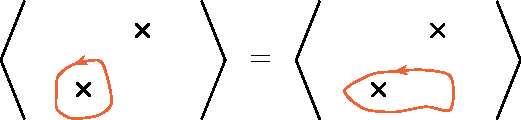
\includegraphics[width=4.16667in,height=\textheight]{figures/tikz/TopOpsDeform.pdf}

}

\caption{\label{fig-TopOpsDeform}Topological operator.}

\end{figure}%

The first goal of this lecture is to understand the following
correspondence:

\begin{tcolorbox}[enhanced jigsaw, opacitybacktitle=0.6, titlerule=0mm, left=2mm, rightrule=.15mm, colbacktitle=quarto-callout-important-color!10!white, coltitle=black, breakable, leftrule=.75mm, bottomtitle=1mm, colback=white, colframe=quarto-callout-important-color-frame, toptitle=1mm, bottomrule=.15mm, opacityback=0, arc=.35mm, title=\textcolor{quarto-callout-important-color}{\faExclamation}\hspace{0.5em}{Symmetry/Topological Operator Correspondence}, toprule=.15mm]

\begin{equation}\phantomsection\label{eq-conv-STO-corresp}{\begin{split}
&\text{(Conventional) locality-preserving symmetry} \\ 
&\Longleftrightarrow\;
\text{invertible topological operator of codimension 1.}
\end{split}
}\end{equation}

\end{tcolorbox}

In this correspondence, the topological operator should be viewed as a
generalization of the \textbf{Noether charge} for potentially discrete
symmetry. More precisely, we consider this correspondence as the
right-hand side \emph{defining} the left-hand side. We will explicitly
verify that this correspondence/definition reproduces the known
symmetries in the case of a classical symmetry in a scalar field theory
in Chapter~\ref{sec-scalar}, and in the case of abelian gauge theory in
Chapter~\ref{sec-vector}. The case of fermions is both intriguing and
crucial, but it will be left as an exercise, or a work, for the
audience/readers.

\begin{tcolorbox}[enhanced jigsaw, opacitybacktitle=0.6, titlerule=0mm, left=2mm, rightrule=.15mm, colbacktitle=quarto-callout-note-color!10!white, coltitle=black, breakable, leftrule=.75mm, bottomtitle=1mm, colback=white, colframe=quarto-callout-note-color-frame, toptitle=1mm, bottomrule=.15mm, opacityback=0, arc=.35mm, title=\textcolor{quarto-callout-note-color}{\faInfo}\hspace{0.5em}{Terminology (Topological Defect)}, toprule=.15mm]

There exists an unfortunate discrepancy in terminology. Outside the
realm of generalized symmetry literature, a ``topological defect''
typically refers to a dynamical object, or its trajectory, viewed as an
operator in the IR theory. As an operator in the IR theory, it is
\emph{not} necessarily topological in the sense of
Figure~\ref{fig-TopOpsDeform}. Conversely, within the generalized
symmetry literature, ``topological defect (operator)'' often signifies
an extended operator that is inherently topological. To mitigate
potential confusion in this lecture, we will adopt the term
``topological operator'', even when the supporting submanifold of the
operator is not within a time-slice.

\end{tcolorbox}

\section{Generalized Symmetry}\label{generalized-symmetry}

The concept of \textbf{generalized (global) symmetry} is fundamentally
based on the correspondence in Equation~\ref{eq-conv-STO-corresp}, as
introduced by \autocite{Gaiotto:2014kfa} \footnote{The concept of global
  higher-form symmetry has been previously explored and investigated in
  the literature, for example, in
  \autocite{Kapustin:2013uxa,Barkeshli:2014cna}. Its gauged version was
  essentially known from \autocite{KalbRamond}.}. This concept expands
the traditional notion of symmetry by loosening the constraints on the
right-hand side of Equation~\ref{eq-conv-STO-corresp}. Hence, we
\emph{define} generalized symmetry through the following correspondence,
which extends Equation~\ref{eq-conv-STO-corresp}:

\begin{tcolorbox}[enhanced jigsaw, opacitybacktitle=0.6, titlerule=0mm, left=2mm, rightrule=.15mm, colbacktitle=quarto-callout-important-color!10!white, coltitle=black, breakable, leftrule=.75mm, bottomtitle=1mm, colback=white, colframe=quarto-callout-important-color-frame, toptitle=1mm, bottomrule=.15mm, opacityback=0, arc=.35mm, title=\textcolor{quarto-callout-important-color}{\faExclamation}\hspace{0.5em}{Generalized Symmetry/Topological Operator Correspondence}, toprule=.15mm]

\begin{equation}\phantomsection\label{eq-GSTO-corresp}{\begin{split}
&\text{Generalized symmetry (in a ``usual" QFT)} \\ 
&\stackrel{\text{def}}{\Longleftrightarrow}\;
\text{General topological operator.}
\end{split}
}\end{equation}

\end{tcolorbox}

In more specific terms, a generalized symmetry that corresponds to an
operator of codimension \(p+1\) is referred to as a \textbf{\(p\)-form
symmetry}. Meanwhile, a generalized symmetry that corresponds to an
operator without an inverse is known as a \textbf{non-invertible
symmetry} (also referred to as category symmetry or topological
symmetry).

In the context of an ``unusual'' QFT, the topological constraint on the
operator in the right-hand side of Equation~\ref{eq-GSTO-corresp} can be
further relaxed. This leads to the concept of \textbf{subsystem}
symmetry, which will be briefly mentioned in
\textbf{?@sec-trivial-scalar}, but will not be discussed in detail in
this lecture.

The table below summarizes the subclasses of generalized symmetry:

\begin{longtable}[]{@{}llll@{}}
\caption{Subclasses of generalized symmetry and defining properties of
their corresponding topological
operators.}\label{tbl-sym-classes}\tabularnewline
\toprule\noalign{}
& \(p\)-form & non-invertible & subsystem \\
\midrule\noalign{}
\endfirsthead
\toprule\noalign{}
& \(p\)-form & non-invertible & subsystem \\
\midrule\noalign{}
\endhead
\bottomrule\noalign{}
\endlastfoot
codimension & \(p+1\) & & \\
Invertible? & & No & \\
Topological? & & & Partially \\
\end{longtable}

These subclasses are not mutually exclusive. Therefore, in theory, a
2-form non-invertible subsystem symmetry could exist, for example.

\section{Contents of the Lecture}\label{contents-of-the-lecture}

\textbf{FIXME}

\bookmarksetup{startatroot}

\chapter{Topological Operators for Classical Symmetry}\label{sec-scalar}

This section explores topological operators in the context of classical
symmetry in scalar field theory.

\section{Set Up}\label{set-up}

For specificity, consider a complex scalar field theory with the
following Lagrangian (density) on a spacetime \(M\) of dimension
\(\stdim\):

\[
\begin{aligned}
\mathcal{L}(\phi) &=  - \left(\frac12 \partial_\mu \phi(x)^* \partial^\nu \phi(x) + V(\phi(x))\right)\vol\\
&= \frac{1}{2} \mathop{d\phi} \wedge *\mathop{d\phi} - V(\phi(x))\vol.
\end{aligned}
\]

In this equation, \(\mathop{*}\) represents the Hodge star,
\(\vol = \mathop{*} 1 = \prod_{i=1}^{\stdim} \mathop{dx_i}\) is the
volume form for the flat space, and \(V(\phi)\) is the potential. Then,
the action is given by:

\[
S[\phi] = \int_{M}\mathcal{L}(\phi).
\]

Consider a symmetry transformation of the scalar field as follows:

\begin{equation}\phantomsection\label{eq-scalar-transf}{
\phi(x) \mapsto \phi^g(x).
}\end{equation}

We assume that this transformation is parametrized by an element \(g\)
in a group \(G\), which is constant over \(M\) and leaves the action
invariant:

\begin{equation}\phantomsection\label{eq-action-inv}{
S[\phi]=S[\phi^g].
}\end{equation}

This implies that the Lagrangian is invariant up to a total derivative:

\begin{equation}\phantomsection\label{eq-Lagrangian-inv}{
\mathcal{L}(\phi^g) = \mathcal{L}(\phi) + \mathop{ds}(\phi,g).
}\end{equation}

In this equation, \(s(\phi,g)\) is a \((\stdim-1)\)-form on \(M\) that
depends on the constant \(g\) and the field \(\phi\). This
\((D-1)\)-form \(s(\phi,g)\) is subject to the ambiguity coming from
shifting by an exact term. Hereafter we use this ambiguity to set
\(s(\phi,\id)=0\).

From the consecutive transformation with \(g_1\) and \(g_2\), we have
\begin{equation}\phantomsection\label{eq-surface-term-assosiative}{ 
s(\phi^{g_1},g_2) + s(\phi,g_1) = s(\phi,g_2g_1) + ds^{(1)}(\phi,g_1,g_2),
}\end{equation} for some \((D-2)\)-form \(s^{(1)}(\phi,g_1,g_2)\). In
particular, setting \(g_2=g_1^{-1}\), we have
\begin{equation}\phantomsection\label{eq-surface-term-inverse}{s(\phi^g,g^{-1}) + s(\phi,g)  = ds^{(1)}(\phi, g, g^{-1}).
}\end{equation} The surface terms \(s\) and \(s^{(1)}\) are related to
\textbf{equivariant cohomology} on the target. See
Appendix~\ref{sec-equivariant} for a further detail.

Here we list two basic examples of classical symmetries. The first one
is the standard \(\U(1)\) rotation corresponds to the transformation:

\[
\phi^g(x) = \mathop{g} \phi(x),
\]

where \(g=e^{\imunit \alpha}\) represents a \(\U(1)\) phase. The
potential \(V(\phi)\) may partially break the \(\U(1)\) rotation into
its subgroup \(\mathbb{Z}_k\). For example, when
\(V(\phi)\propto \phi^k+(\phi^*)^k\), the parameter \(g\) takes
\emph{discrete} values: \(g = e^{\imunit \frac{2\pi p}{k}}\), for an
integer \(p\).

Moreover, when \(V(\phi)=0\), the action \(S[\phi]\) also admits the
shift symmetry\footnote{If we use the form of the Lagrangian
  \(\mathcal{L}^\prime= -\frac12 \phi \mathop{d*d\phi}\), this provides
  an example where the total derivative in
  Equation~\ref{eq-Lagrangian-inv} is nonzero:
  \(s=-\frac12 \alpha \mathop{*}\mathop{d\phi}\).}:

\[
\phi^{\alpha}(x) = \phi(x) + \alpha.
\]

In the rest of this section, our goal is to construct the
\textbf{topological operator} corresponding to these \emph{classical}
symmetries.

\begin{tcolorbox}[enhanced jigsaw, opacitybacktitle=0.6, titlerule=0mm, left=2mm, rightrule=.15mm, colbacktitle=quarto-callout-note-color!10!white, coltitle=black, breakable, leftrule=.75mm, bottomtitle=1mm, colback=white, colframe=quarto-callout-note-color-frame, toptitle=1mm, bottomrule=.15mm, opacityback=0, arc=.35mm, title=\textcolor{quarto-callout-note-color}{\faInfo}\hspace{0.5em}{Note}, toprule=.15mm]

This construction can be applied to various types of scalar field
theory, such as real and/or multiple scalar fields, provided the kinetic
term is standard enough (more details in Tip~\ref{tip-fracton}). Also
note that the spacetime manifold \(M\) and its metric do not need to be
flat. The metric's signature is not significant in this lecture, even
though we use Euclidean notation.

\end{tcolorbox}

\begin{tcolorbox}[enhanced jigsaw, opacitybacktitle=0.6, titlerule=0mm, left=2mm, rightrule=.15mm, colbacktitle=quarto-callout-note-color!10!white, coltitle=black, breakable, leftrule=.75mm, bottomtitle=1mm, colback=white, colframe=quarto-callout-note-color-frame, toptitle=1mm, bottomrule=.15mm, opacityback=0, arc=.35mm, title=\textcolor{quarto-callout-note-color}{\faInfo}\hspace{0.5em}{Note}, toprule=.15mm]

In this lecture, we focus on constructing topological operators that
correspond to the \emph{finite} transformation
Equation~\ref{eq-scalar-transf}, as opposed to the conventional approach
of considering infinitesimal transformations. This approach allows us to
explicitly discuss \emph{discrete} symmetries (and their anomalies) in
terms of topological operators, and it also motivates us to consider
generalized symmetries.

\end{tcolorbox}

\section{Construction of the Topological
Operator}\label{construction-of-the-topological-operator}

As a fundamental example of the correspondence
Equation~\ref{eq-conv-STO-corresp}, we aim to construct the topological
operator \(U_\alpha[W]\) that corresponds to the transformation
Equation~\ref{eq-scalar-transf}. Specifically, we will construct an
operator \(U_\alpha[W]\), defined on a codimension-1 submanifold \(W\)
of the spacetime \(M\), that satisfies the following properties:

\begin{tcolorbox}[enhanced jigsaw, opacitybacktitle=0.6, titlerule=0mm, left=2mm, rightrule=.15mm, colbacktitle=quarto-callout-important-color!10!white, coltitle=black, breakable, leftrule=.75mm, bottomtitle=1mm, colback=white, colframe=quarto-callout-important-color-frame, toptitle=1mm, bottomrule=.15mm, opacityback=0, arc=.35mm, title=\textcolor{quarto-callout-important-color}{\faExclamation}\hspace{0.5em}{Properties of the Symmetry Topological Operator}, toprule=.15mm]

\begin{enumerate}
\def\labelenumi{\arabic{enumi}.}
\tightlist
\item
  Topological: \(U_g[W] = U_g[W']\) if \(W\) can be continuously
  deformed into \(W'\) without intersecting other operators.
\item
  Symmetry action: When a deformation from \(W\) to \(W''\) intersects a
  local operator \(\mathcal{O}\), it undergoes the symmetry action
  specified by \(g\), resulting in another operator \(\mathcal{O}^g\).
\item
  Noether: When the symmetry group is continuous, we can consider the
  group element as the infinitesimal deformation of \(\id\):
  \(g = \id + \alpha + \mathcal{O}(\alpha^2)\). In this case, the
  operator \(U_g[W]\) is approximated by the Noether charge
  \begin{equation}\phantomsection\label{eq-Noether-approx}{
   U_{1+\alpha+\mathcal{O}(\alpha^2)} = 1 + \alpha \int_W \mathop{*}j +\mathcal{O}(\alpha^2),
   }\end{equation} where \(j = j_\mu\mathop{dx^\mu}\) is the Noether
  current one-form. \textbf{FIXME:sign is uncertain..} \[
   \mathop{*}j = \left.\frac{\delta\mathcal{L}(\phi^{1+\alpha(x)})}{\delta d\alpha}\right|_{\alpha=0} + \left.\frac{\partial s(\phi, 1+ \alpha)}{\partial \alpha}\right|_{\alpha=0}.
   \] Note that when \(W\) is a time-slice \(W=\{t=0\}\), \[
  \int_W \mathop{*} j = \int_{\{t=0\}} j^0 \mathop{d^{\stdim-1}x}
  \] is precisely the Noether charge as described in any QFT textbook.
\end{enumerate}

Properties 1 and 2 are summarized in Figure~\ref{fig-op-action}.

\end{tcolorbox}

\begin{figure}[t]

\centering{

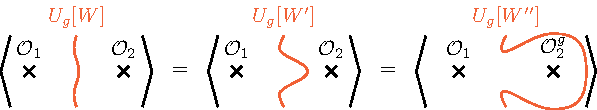
\includegraphics[width=4.16667in,height=\textheight]{figures/tikz/Op_action.pdf}

}

\caption{\label{fig-op-action}The topological operator \(U_g[W]\) is
designed to be invariant under a continuous deformation and to implement
the symmetry action.}

\end{figure}%

The construction is based on the concept of
``cutting-and-gluing-with-twist''. Initially, we partition the spacetime
\(M\) into two subregions: \(M_\stdim = M_L \cup_W M_R\) with a common
boundary \(W\) (refer to Figure~\ref{fig-cut-M}. We orient \(W\) such
that \(\partial M_L = -\partial M_R = W\).). We also divide the scalar
field \(\phi\) into two fields: \(\phi_L(x)\) for \(x \in M_L\) and
\(\phi_R(x)\) for \(x \in M_R\). Subsequently, we reconnect the two
regions and their respective fields, with a twisted identification:
\[ \phi_L|_W = \phi_R^{g^{-1}}|_W. \]

\begin{figure}[t]

\centering{

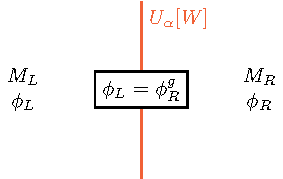
\includegraphics[width=2.39583in,height=\textheight]{figures/tikz/ManifoldSplit.pdf}

}

\caption{\label{fig-cut-M}The cutting and twisted gluing, implementing
the topological operator \(U_g[W]\).}

\end{figure}%

In path-integral, this construction can be implemented as follows:

\begin{tcolorbox}[enhanced jigsaw, opacitybacktitle=0.6, titlerule=0mm, left=2mm, rightrule=.15mm, colbacktitle=quarto-callout-important-color!10!white, coltitle=black, breakable, leftrule=.75mm, bottomtitle=1mm, colback=white, colframe=quarto-callout-important-color-frame, toptitle=1mm, bottomrule=.15mm, opacityback=0, arc=.35mm, title=\textcolor{quarto-callout-important-color}{\faExclamation}\hspace{0.5em}{Symmetry Topological Operator for a Classical Symmetry}, toprule=.15mm]

\begin{equation}\phantomsection\label{eq-Ug-pathintegral}{
\begin{multlined}
    \langle U_g[W] \cdots \rangle = \int \mathop{\mathcal{D}^{M_L}\phi_L} \mathop{\mathcal{D}^{M_R}\phi_R} \mathop{\mathcal{D}^W\lambda} \cdots\\ \times \exp\left(-S_L[\phi_L]-S_R[\phi_R] - G_W[\lambda,\phi_L,\phi_R,g]\right)
\end{multlined}
}\end{equation}

\end{tcolorbox}

Here, \(\mathcal{D}^{X}\) denotes the measure for the path-integral for
a field defined on a submanifold \(X\) of the spacetime \(M\). The
actions on the submanifold \(M_{L,R}\) are written as
\(S_{L,R} = \int_{M_{L,R}}\mathcal{L}(\phi_{L,R})\), and ``\(\cdots\)''
denotes additional operator insertions. The ``gluing'' action \(G_W\) on
the submanifold \(W\) is defined as
\begin{equation}\phantomsection\label{eq-gluing-action}{
%\begin{multlined}
    G_W[\lambda,\phi_L,\phi_R,g] = - \imunit \int_W \lambda(\phi_L - \phi_R^{g^{-1}})\vol_W+\int_W s(\phi_R^{g^{-1}},g).
%\end{multlined}
}\end{equation} The key point of the above expression is that
integrating the Lagrange multiplier \(\lambda\) results in the ``delta
functional'':
\begin{equation}\phantomsection\label{eq-delta-functional}{
    \int \mathop{\mathcal{D}^W\lambda} \exp\left(\imunit \int_W \lambda (\phi_L-\phi^{g^{-1}}_R)\vol_W\right)
     = \prod_{x\in W}\delta(\phi_L(x) - \phi_R^{g^{-1}}(x)),
}\end{equation} which should implement Figure~\ref{fig-cut-M}. Before
studying the operator \(U_g[W]\), we should first examine the
\emph{trivial} case where the symmetry transformation \(g\) is the
identity map \(g=\id\).
\begin{equation}\phantomsection\label{eq-identity-wall}{
\langle \id[W] \cdots \rangle = \langle \cdots \rangle.
}\end{equation} We refer to the codimension-1 operator \(\id[W]\) with
this property as the \textbf{identity wall}. It can also be termed as
the \textbf{transparent wall} or similar. Upon expanding
Equation~\ref{eq-identity-wall}, the following equation should be
satisfied: \begin{equation}\phantomsection\label{eq-trivial-scalar}{
\begin{multlined}
    \int \mathop{\mathcal{D}^M\phi} \exp(-S) \cdots=
    \int \mathop{\mathcal{D}^{M_L}\phi_L} \mathop{\mathcal{D}^{M_R}\phi_R} \mathop{\mathcal{D}^W\lambda} \\ \times \exp\left(-S_L-S_R+\imunit \int_W \lambda(\phi_L - \phi_R)\vol_W\right)\cdots.\\ 
\end{multlined}
}\end{equation}

The key distinction between providing a field \(\phi\) on \(M\) and
providing a pair of fields \((\phi_L,\phi_R)\) on \((M_L,M_R)\) is that
the latter is not required to be continuous across \(W\). On the
right-hand side, continuity is enforced by integrating out \(\lambda\)
due to Equation~\ref{eq-delta-functional}.

\begin{tcolorbox}[enhanced jigsaw, opacitybacktitle=0.6, titlerule=0mm, left=2mm, rightrule=.15mm, colbacktitle=quarto-callout-tip-color!10!white, coltitle=black, breakable, leftrule=.75mm, bottomtitle=1mm, colback=white, colframe=quarto-callout-tip-color-frame, toptitle=1mm, bottomrule=.15mm, opacityback=0, arc=.35mm, title=\textcolor{quarto-callout-tip-color}{\faLightbulb}\hspace{0.5em}{Tip \ref*{tip-fracton}: Continuity of Fields in ``Exotic'' QFTs and Subsystem Symmetry}, toprule=.15mm]

\quartocallouttip{tip-fracton} 

In this context, we assume that the path integral
\(\int\mathcal{D}^M\phi\) should be over the \emph{continuous} fields.
This is because the standard kinetic term would diverge when the field
\(\phi\) becomes discontinuous, and thus such configuration does not
contribute to the path-integral.

However, this assumption does not hold for QFTs with higher-derivative
kinetic terms. Examples of such exotic QFTs (without relativistic
symmetry) include tensor gauge theories (refer to
\autocite{Pretko:2020cko,Seiberg:2020bhn} for more details). An example
of such kinetic term is
\((\partial_t\phi)^2 + (\partial_x\partial_y \phi)^2\). In these
theories, a field \emph{can} be discontinuous, but some higher
derivatives are constrained to scale appropriately with the ratio of the
lattice size to the system size. In such scenarios, the construction of
the trivial operator should differ.

These QFTs describe what is known as the \textbf{fracton phases} of
matter, which do not have emergent continuous rotational symmetry in the
IR. Moreover, these models typically possess \textbf{subsystem
symmetries}, whose corresponding operator is not entirely topological.
The existence of this new type of symmetry, absent in standard
relativistic systems, could be related to this subtlety regarding
identity wall .

\end{tcolorbox}

Let us study the equations of motion (EOMs) on the right-hand side of
Equation~\ref{eq-trivial-scalar}. The EOM with respect to \(\lambda\)
simply enforces \(\phi_L(x) = \phi_R(x)\) for \(x\in W\). On the other
hand, the surface term of the Euler-Lagrange equation for \(\phi_L\) and
\(\phi_R\) yields \[
    \left.\frac{\delta \mathcal{L}[\phi_L]}{\delta \mathop{d\phi_L}}\right|_W = \lambda \vol_W = \left. \frac{\delta \mathcal{L}[\phi_R]}{\delta \mathop{d \phi_R}}\right|_W.
\] If \(W\) is spacelike, or if we interpret the direction perpendicular
to \(W\) as the imaginary time in Euclidean signature, this condition
ensures the continuity of the canonical momentum across \(W\).

\begin{tcolorbox}[enhanced jigsaw, opacitybacktitle=0.6, titlerule=0mm, left=2mm, rightrule=.15mm, colbacktitle=quarto-callout-note-color!10!white, coltitle=black, breakable, leftrule=.75mm, bottomtitle=1mm, colback=white, colframe=quarto-callout-note-color-frame, toptitle=1mm, bottomrule=.15mm, opacityback=0, arc=.35mm, title=\textcolor{quarto-callout-note-color}{\faInfo}\hspace{0.5em}{Locality}, toprule=.15mm]

Equation~\ref{eq-trivial-scalar} encapsulates the \textbf{locality} of
the path-integral. We can employ the same procedure to decompose the
path-integral \(\int \mathcal{D}^M{\phi}\) on \(M\) into path-integrals
on local patches, like \(\int \prod_i\mathcal{D}^{V_i}\phi_i\)
(accompanied by numerous Lagrange multipliers). Here,
\(\bigcup_i V_i =M\) and \(V_i \cap V_j\) has codimension 1 in \(M\) if
not empty.

In the realm of topological quantum field theory (TQFT), a similar
\textbf{cutting-and-gluing} axiom is utilized in the Atiyah-Segal
formulation of topological quantum field theory. Later, Lurie's
cobordism hypothesis \autocite{Lurie} established the relationship
between this axiom and locality.

\end{tcolorbox}

\begin{tcolorbox}[enhanced jigsaw, opacitybacktitle=0.6, titlerule=0mm, left=2mm, rightrule=.15mm, colbacktitle=quarto-callout-tip-color!10!white, coltitle=black, breakable, leftrule=.75mm, bottomtitle=1mm, colback=white, colframe=quarto-callout-tip-color-frame, toptitle=1mm, bottomrule=.15mm, opacityback=0, arc=.35mm, title=\textcolor{quarto-callout-tip-color}{\faLightbulb}\hspace{0.5em}{A note on fermions}, toprule=.15mm]

While this lecture does not cover fermions, it's worth noting how they
would differ in this context.

In scalar field theory, we enforce the continuity of the ``position''
variables (in the analytical-mechanical sense) \(\phi\), and the
continuity of the momentum variables follows from the equations of
motion (EOM).

However, in a chiral fermion theory, the kinetic term involves only one
derivative, making it typically impossible to separate position and
momentum variables while preserving Lorentz or global chiral symmetry.
Consequently, the ``cutting'' process would seemingly violate invariance
under Lorentz or another symmetry, which can be interpreted as a
manifestation of the gravitational and global symmetry anomaly. A
precise understanding of this perspective is beyond the scope of this
lecture.

\end{tcolorbox}

\section{Topological-ness}\label{topological-ness}

Let us show the topological-ness of \(U_g\), i.e.~the first equation in
Figure~\ref{fig-op-action}, or
\begin{equation}\phantomsection\label{eq-U-top}{
U_{g}[W_1]\id[W_2] = \id[W_1]U_{g}[W_2].
}\end{equation} To show Equation~\ref{eq-U-top}, we divide the spacetime
into three parts: \(M_L,M_M\) and \(M_L\), where \(W\) separates \(M_L\)
and \(M_M\), while \(W'\) separates \(M_M\) and \(M_R\). The relevant
part of paht-integral regarding the left hand side of
Equation~\ref{eq-U-group} reads \[
\int\mathcal{D}^{M_M}\phi_M\mathcal{D}^{W_1}\lambda_1\mathcal{D}^{W_2}\lambda_2 \, e^{-S_M[\phi_M]-G_{W_1}[\phi_L,\phi_M,g]-G_{W_2}[\phi_M,\phi_R,\id]}.
\] Here \(S_M = \int_{M_M}\mathcal{L}[\phi_M]\) and we omit the
path-integral measures for \(\phi_{L,R}\) and also the actions on
\(M_L\) and \(M_R\) for the sake of readability. By changing the
variable by \(\tilde{\phi}_M^{g} = \phi_M\), we get the expression \[
\int\mathcal{D}^{M_M}\tilde{\phi}_M^g\mathcal{D}^{W_1}\lambda_1\mathcal{D}^{W_2}\lambda_2 \, e^{-S_M[\tilde\phi_M^g]-G_{W_1}[\lambda_1,\phi_L,\phi_M,\id] - \int_{W_1} s(\tilde\phi_M,g) -G_{W_2}[\lambda_2,\tilde\phi_M^g,\phi_R,\id]}.
\] As \(M_M\) is open, the action \(S_M[\tilde\phi_M^g]\) catches up the
surface term: \[
S_M[\tilde\phi_M^g] = S_M[\tilde\phi_M] - \int_{W_1} s(\tilde{\phi}_M,g) + \int_{W_2} s(\tilde{\phi}_M,g).
\] Using this equation combined with
Equation~\ref{eq-surface-term-inverse}, we get \[
\int\mathcal{D}^{M_M}\tilde{\phi}_M^g\mathcal{D}^{W_1}\lambda_1\mathcal{D}^{W_2}\lambda_2 \, e^{-S_M[\tilde\phi_M^g]-G_{W_1}[\lambda_1,\phi_L,\tilde\phi_M,\id] -G_{-W_2}[\lambda_2,\phi_R,\tilde\phi_M,g^{-1}]},
\] where \(-W_2\) is the orientation reversal of \(W_2\). Then we use
the invariance of the path-integral measure of the sclar fields (up to
the overall nomarlization):
\begin{equation}\phantomsection\label{eq-measure-inv}{\mathcal{D}^{M_M}\phi_M = \mathcal{D}^{M_M}\phi_M^g
}\end{equation} to get \[
U_{g}[W_1]= U_{g^{-1}}[-W_2].
\]

Lastly, we need to show
\begin{equation}\phantomsection\label{eq-Udual-inverse}{ U_{g^{-1}}[-W] = U_g[W].
}\end{equation} To show this, we assume that there exists a
transformation \(\lambda^g\) of \(\lambda\) that satisfies
\[ \lambda(\phi_L-\phi_R) = \lambda^{g}(\phi_L^{g}-\phi_R^{g})
\] and \[ \mathcal{D}^W\lambda^g = \mathcal{D}^W\lambda. 
\] For example, when the action is a \(\U(1)\) rotation \(\lambda^g\) is
the rotation by the inverse, and when the action is a shift of \(\phi\),
we can set \(\lambda^g = \lambda\). Then, \[
\begin{split}
U_{g^{-1}}[-W] &= \int\mathcal{D}^W \lambda \, e^{-G_{-W}[\lambda^{g^{-1}},\phi_R,\phi_L,g^{-1}]}\\
&= \int\mathcal{D}^W \lambda \, e^{\imunit\int_{-W}\lambda(\phi_R-\phi_L^{g})\vol_W - \int_{-W}s(\phi_L^{g},g^{-1})}\\
&= \int\mathcal{D}^W \lambda \, e^{\imunit\int_{W}\lambda^{g^{-1}}(\phi_L-\phi_R^{g^{-1}})\vol_W - \int_{W}s(\phi_L,g)}\\
&= \int\mathcal{D}^W \lambda^{g^{-1}} \, e^{-G_W[\lambda^{g^{-1}},\phi_L,\phi_R,g]}\\
&= U_g[W].
\end{split}
\]

We note that we can also get the following equation in the same way as
above: \begin{equation}\phantomsection\label{eq-bubble}{
\langle \mathcal{O}_1 \mathcal{O}_2 \cdots \rangle = \langle U_g[W_0] \mathcal{O}_1 \mathcal{O}_2 \cdots \rangle,
}\end{equation} when \(W_0\) encloses a compact region of \(M\) and
contains no operator.

\section{Group Multiplication Law and
Junction}\label{group-multiplication-law-and-junction}

For the conventional symmetry, we assume that transformations \(g\)
forms a group. Correspondingly, the topological operators should satisfy
the same multiplication law:
\begin{equation}\phantomsection\label{eq-U-group}{
U_{g_1}[W_1] U_{g_2}[W_2] = U_{g_1g_2}[W_1]
}\end{equation} where the codimension-1 submanifold \(W_2\) is parralel
to \(W_1\) but slightly right to it. One can show this in the same
manner we have done for Equation~\ref{eq-U-top}. In particular, from
Equation~\ref{eq-Udual-inverse} we have
\begin{equation}\phantomsection\label{eq-Udual-inverse-2}{ U_g[W_1] U_g[-W_2] = U_g[W_1] U_{g^{-1}}[W_2] = U_{\id}[W_1] = \id[W_1].
}\end{equation} That is, the orientation reversal of \(U_g\) is its
inverse. The properties Equation~\ref{eq-U-group} and
Equation~\ref{eq-Udual-inverse-2} are the properties of a conventional
symmetry and will be relatex in a generalized --- specifically
non-invertible --- symmetry.

For later convenience, here we also introduce the \textbf{topological
junctions} of topological operators \(U_{g_1},U_{g_2},U_{g_3}\). A
junction is the object connecting multiple extended operators. For the
classical symmetry, such an junction is defined by putting three (or
more) operators on submanifolds \(W_1,W_2\) and \(W_3\) sharing their
boundary \(X\): \[
U_{g_1}[W_1]U_{g_2}[W_2]U_{g_3}[W_3]J_{g_1,g_2,g_3}[X] 
=
\int\prod_{i=1}^3\mathcal{D}^{W_i}\lambda_i
\, e^{-\sum_i G_{W_i}[\lambda_i,\phi_i,\phi_{i+1},g_i]-\int_X s^{(1)}(\phi_1,g_1,g_2)},
\] which can be proven to be topological when \(g_3=g_1g_2\).
\textbf{FIGURE} \textbf{Example of nonzero \(s^{(1)}\) or higher?}

\section{Symmetry Action and Ward-Takahashi
identity}\label{symmetry-action-and-ward-takahashi-identity}

When we have local operator in addition to topological symmetry
operators, we also need the second equation in
Figure~\ref{fig-op-action}, or the equation \[
U_g[W_1] \mathcal{O} = \mathcal{O}^g U_g[W_2],
\] where \[\mathcal{O}^g[\phi] := \mathcal{O}[\phi^g]
\] is the local operator acted by \(g \in G\). This equation follows
from the same manipulation as that proved Equation~\ref{eq-U-top}, but
with an operator insertion in the region \(M_M\).

Then, by repeatedly using these equations, we get the
\textbf{Ward-Takahashi identity} :

\begin{tcolorbox}[enhanced jigsaw, opacitybacktitle=0.6, titlerule=0mm, left=2mm, rightrule=.15mm, colbacktitle=quarto-callout-important-color!10!white, coltitle=black, breakable, leftrule=.75mm, bottomtitle=1mm, colback=white, colframe=quarto-callout-important-color-frame, toptitle=1mm, bottomrule=.15mm, opacityback=0, arc=.35mm, title=\textcolor{quarto-callout-important-color}{\faExclamation}\hspace{0.5em}{Ward-Takahashi Identity}, toprule=.15mm]

\begin{equation}\phantomsection\label{eq-Ward-Takahashi}{
\begin{aligned}
\langle \mathcal{O}_1 \mathcal{O}_2 \cdots \mathcal{O}_N \rangle
&= 
\langle U_g[W_0] \mathcal{O}_1 \mathcal{O}_2 \cdots \mathcal{O}_N \rangle\\
&= 
\langle \mathcal{O}_1^g U_g[W_1] \mathcal{O}_2 \cdots \mathcal{O}_N \rangle\\
&= 
\langle \mathcal{O}_1^g  \mathcal{O}_2^g \cdots \mathcal{O}_N^g U_g[W_N] \rangle\\
&= 
\langle \mathcal{O}_1^g  \mathcal{O}_2^g \cdots \mathcal{O}_N^g\rangle,
\end{aligned}
}\end{equation} where \(W_i\) encloses the operators
\(\mathcal{O}_1 \cdots \mathcal{O}_i\), and at the last step we
collapsed \(U_g[W_N]\) towards the infinity (or whatever point if \(M\)
is compact). See also Figure~\ref{fig-Ward-Takahashi}.

\end{tcolorbox}

\begin{figure}[t]

\centering{

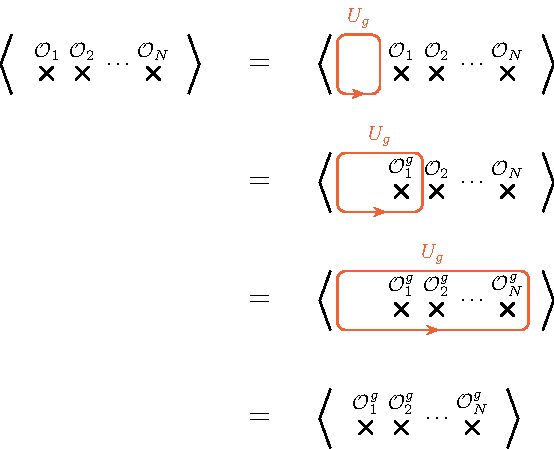
\includegraphics[width=4.16667in,height=\textheight]{figures/tikz/WardTakahashi.pdf}

}

\caption{\label{fig-Ward-Takahashi}Derivation of Ward-Takahashi identity
Equation~\ref{eq-Ward-Takahashi}.}

\end{figure}%

We could get the same result by considering global change of variable
\(\widetilde{\phi} = \phi^{g^{-1}}\) in the path-integral and could
avoid topological operator to derive this identity. However, the
deriviation in Figure~\ref{fig-Ward-Takahashi} applies as long as we
have a topological operator, and it acts on local operators as in
Figure~\ref{fig-op-action}. Thus this derivation is applicable to
quantum and duality symmetry we will encounter in
Chapter~\ref{sec-compact-boson}, and also will be convenient starting
point to generalizing the identity to non-invertible case; see
\textcite{Cordova:2022ieu} and \textcite{Copetti:2023mcq} for example.

Let us quickly recall that Ward-Takahashi identity means selection rules
in correlation functions. For simplicity, let us consider the \(\U(1)\)
action: \begin{equation}\phantomsection\label{eq-WT-U1}{
\mathcal{O}_i^g = g^{q_i}\mathcal{O}_i
}\end{equation} for a phase \(g \in \U(1)\). The integer \(q_i\) is the
\(\U(1)\) globalcharge of \(\mathcal{O}_i\). In this case,
Equation~\ref{eq-Ward-Takahashi} reads \[ 
\left(1-g^{\sum_i q_i}\right)\left\langle \prod_i \mathcal{O}_i\right\rangle = 0,
\] for any phase \(g \in \U(1)\). That is, either \(\sum_i q_i =0\) ---
the total \(\U(1)\) charge is saturated --- or that the correlation
function vanishes. This is the familiar selection rule. If the \(\U(1)\)
symmetry is broken down to its \(\mathbb{Z}_k\) subgroup,
Equation~\ref{eq-WT-U1} holds only for \(g\in \mathbb{Z}_k\). This means
the total charge \(\sum_i q_i\) should vanish only modulo \(k\) for the
correlator to be nonzero.

\begin{tcolorbox}[enhanced jigsaw, opacitybacktitle=0.6, titlerule=0mm, left=2mm, rightrule=.15mm, colbacktitle=quarto-callout-tip-color!10!white, coltitle=black, breakable, leftrule=.75mm, bottomtitle=1mm, colback=white, colframe=quarto-callout-tip-color-frame, toptitle=1mm, bottomrule=.15mm, opacityback=0, arc=.35mm, title=\textcolor{quarto-callout-tip-color}{\faLightbulb}\hspace{0.5em}{Mixed-gravitational anomaly}, toprule=.15mm]

The symmetry we discuss here does not suffer from anomaly and the
Ward-Takahashi idendity (Equation~\ref{eq-Ward-Takahashi}) follows. If
we instead consider the topological operator corresponding to a symmetry
with mixed-gravitational anomaly, the invariance of the measure
(Equation~\ref{eq-measure-inv}) does not necessarily hold when \(M_M\)
does not have the topology of a ball, and likewise
Equation~\ref{eq-bubble} can fail when \(W_0\) is not a ball. Thus, on a
spacetime with non-trivial topology (other than \(\mathbb{R}^4\) or
\(S^4\)), (Equation~\ref{eq-Ward-Takahashi}) might fail at the last
equality, while (by choosing \(W_0\) to be a ball) other steps goes
through. The failure is by a phase depending on topology of the
spacetime, and has an interesting consequences of this discussed in
\autocite{Cordova:2019jqi}.

\end{tcolorbox}

\section{Relation to Noether Charge}\label{relation-to-noether-charge}

Here we show the relation Equation~\ref{eq-Noether-approx} of the
topological operator \(U_g[W]\) to the conventional Noether charge. This
can be done by applying the change of variable
\(\widetilde{\phi_R} = \phi^{\id - \alpha f(x_n)}_R\) to
Equation~\ref{eq-Ug-pathintegral}, where \(f(x_n,\delta)\) is a function
of the coordinate \(x_n\) perpendicular to \(W\) and one positive
parameter \(\delta\) and satisfies \(f(0) = 1\) and
\(f(x_n>\delta) =0\). Then we take \(\delta\to 0\) limit and compare.
\textbf{FIXME:write equations}

\bookmarksetup{startatroot}

\chapter{Compact Boson}\label{sec-compact-boson}

Here we consider \emph{compact} boson, where the field \(\phi\) is real
and subject to the identification \[
\phi(x) \cong \phi(x) + 2\pi.
\] We take the Lagrangian to be \[
\mathcal{L} = \frac{R^2}{4\pi}\int_M \mathop{d\phi} \wedge \mathop{*}\mathop{d\phi}.
\] We can normalize the field \(\phi\) so that it has the kinetic term
with a fixed coefficient, in which case the normalized field has a
periodicity radius proportional to \(R\).

The theory has the shift (or ``momentum'') \(\U(1)\) symmetry \[
\phi^\alpha = \phi + \alpha 
\] with identification of the parameter \(\alpha \cong \alpha + 2\pi\).
One can add a periodic potential \(V(\phi)\) and restrict oneself to a
discrete symmetry preserving the potential.

In addition to the shift symmetry, the system has other generalized
symmetries:

\begin{enumerate}
\def\labelenumi{\arabic{enumi}.}
\tightlist
\item
  \textbf{winding} \(\U(1)\) (\(\stdim-2\))-form symmetry
  \autocite{Gaiotto:2014kfa}, and
\item
  when \(\stdim=2\) and \(R^2\) is rational, there exists a
  \textbf{T-duality} symmetry that is in general \emph{non-invertible}
  \autocites{Choi:2021kmx}{Niro:2022ctq}{Cordova:2023ent,Nagoya:2023zky}.
\end{enumerate}

The purpose of this section is to understand these generalized
symmetries, but before that we review the shift symmetry.

\section{Trivial Operator and Shift Symmetry
Operator}\label{trivial-operator-and-shift-symmetry-operator}

We start from the identity operator \(\id[W^{\stdim-1}]\) that cuts and
glues the path-integral. The construction is almost the same as before,
but when we glue the fields \(\phi_L\) and \(\phi_R\) along
\(W^{\stdim-1}\), the gluing can be up to a integer multiple of
\(2\pi\): \[
    \phi_L(x) = \phi_R(x) + 2\pi n 
\] with an integer \(n\) (assuming \(W^{\stdim-1}\) is connected).
Therefore, the gluing part of the path-integral is \[
\id[W^{\stdim-1}] = \sum_{n\in\mathbb{Z}}\int \mathcal{D}^{W^{\stdim-1}}\lambda \exp\left(\imunit\int_{W^{\stdim-1}} \lambda\left(\phi_L-\phi_R - 2\pi n\right)\right)\vol_{W^{\stdim-1}}.
\] We can sum \(n\) out to restrict \(\lambda\) to satisfy \[
    \int_{W^{\stdim-1}}\lambda \vol_{W^{\stdim-1}} \in \mathbb{Z}.
\] An integration over such lambda can be replaced by integration in
terms of \((\stdim-2)\)-form \(\U(1)\) gauge field \(V\) with \[
\mathop{dV} = 2\pi \lambda\vol_{W^{\stdim-1}}.
\] Therefore the identity operator can be written as\footnote{We assume
  that the integration should be done over \emph{gauge equivalent
  classes} of \(V\). In other words the gauge fixing procedure is
  implicit in this lecture.}
\begin{equation}\phantomsection\label{eq-identity-compact-boson}{
    \id[{W^{\stdim-1}}] = \int \mathcal{D}^{W^{\stdim-1}}V \exp\left(\frac{\imunit}{2\pi}\int_{W^{\stdim-1}} \mathop{dV}\left(\phi_L-\phi_R\right)\right).
}\end{equation}

\begin{tcolorbox}[enhanced jigsaw, opacitybacktitle=0.6, titlerule=0mm, left=2mm, rightrule=.15mm, colbacktitle=quarto-callout-note-color!10!white, coltitle=black, breakable, leftrule=.75mm, bottomtitle=1mm, colback=white, colframe=quarto-callout-note-color-frame, toptitle=1mm, bottomrule=.15mm, opacityback=0, arc=.35mm, title=\textcolor{quarto-callout-note-color}{\faInfo}\hspace{0.5em}{\(p\)-form gauge field}, toprule=.15mm]

A \(p\)-form gauge field \(V\) is \emph{locally} (i.e.~in a patch)
\(p\)-form, but \(V\) is not necessarily a \emph{global} \(p\)-form and
\(\mathop{dV}\) rather satisfy
\(\int_{\Sigma_{p+1}}\mathop{dV}\in 2\pi \mathbb{Z}\) for any \(p+1\)
dimensional submanifold.

If a reader is not familiar with this concept, one can assume
\(\stdim = 2,3\). When \(\stdim=3\), \(V\) is a usual (one-form) abelian
gauge field, whose magnetic flux is quantized, while when \(\stdim =2\),
\(V\) is a periodic scalar field. About higher-form gauge field, a
motivated reader can consult e.g.~\textcite{Hsieh:2020jpj}.

\end{tcolorbox}

Now the topological operator for the shift symmetry is simply
\begin{equation}\phantomsection\label{eq-shift-compact-boson}{
    U_\alpha^\text{shift}[{W^{\stdim-1}}] = \int \mathcal{D}^{W^{\stdim-1}}V \exp\left(\frac{\imunit}{2\pi}\int_{W^{\stdim-1}} \mathop{dV}\left(\phi_L-\phi_R + \alpha\right)\right).
}\end{equation}

\section{Winding Symmetry}\label{winding-symmetry}

The compact boson theory has another topological operator of dimension 1
(codimension \(\stdim-1\)), which is simply
\begin{equation}\phantomsection\label{eq-winding-op}{
U^\text{winding}_\alpha[\gamma^1] = \exp\left(\imunit\alpha \int_{\gamma^1}\frac{\mathop{d\phi}}{2\pi}\right).
}\end{equation} Given the periodicity, the integral
\(\int_{\gamma^1}\mathop{d\phi}\) for a closed \(\gamma^1\) takes a
value in \(2\pi \mathbb{Z}\), and therefore the operator is invariant
against deformation of \(\gamma^1\). This also indicates that the
parameter \(\alpha\) is \(2\pi\) periodic. According to
Table~\ref{tbl-sym-classes}, this topological operator should define a
\(\U(1)\) \(p\)-form symmetry with \(p=(\stdim-2)\), called the
\textbf{winding symmetry}.

What are the operators \emph{charged} under the symmetry? When
\(p \ge 1\) (\(\stdim\ge 3\)), the operator Equation~\ref{eq-winding-op}
cannot act on a local (point) operator, because the one-dimensional
submanifold \(\gamma^1\) can always be deformed one configuration to
another without colliding with a point. On the other hand, it can
potentially act on a \(p\)-dimensional extended operator:
Figure~\ref{fig-one-form}.

\begin{figure}[t]

\begin{minipage}{0.50\linewidth}
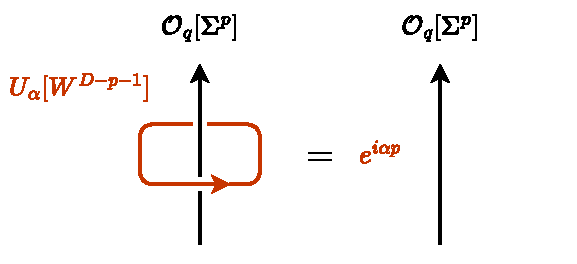
\includegraphics{figures/one-form_act.pdf}\end{minipage}%
%
\begin{minipage}{0.50\linewidth}
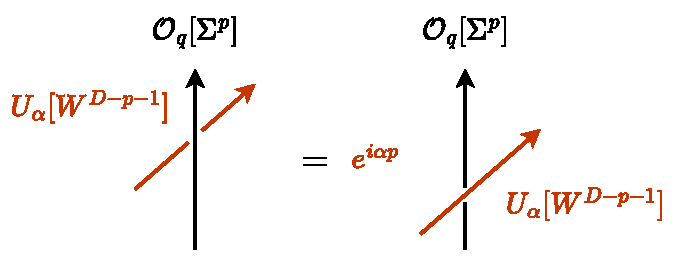
\includegraphics{figures/one_form_passing.pdf}\end{minipage}%

\caption{\label{fig-one-form}Action of \(p\)-form symmetry operator
\(U_\alpha[W^{D-p-1}]\) on a \(p\)-dimensional operator
\(\mathcal{O}_q[\Sigma^p]\) of \(p\)-form charge \(q\). We can consider
the two types of actions, one is \emph{encircling} action (left), and
the other is the \emph{passing} action (right). From the latter we can
close the loop on the right of the \(\mathcal{O}_q\), and contract the
loop on the right hand side, to get the former type of action.}

\end{figure}%

However, the construction of a charged operator is a bit tricky. A way
of doing it is to first insert the identity operator
Equation~\ref{eq-identity-compact-boson}, then utilize the field \(V\)
on the identity operator to defing an operator charged under
Equation~\ref{eq-winding-op}. Concretely, the (non-topological) operator
with winding charge \(n\) can be constructed as
\begin{equation}\phantomsection\label{eq-dual-op}{
\langle \mathcal{O}^\text{winding}_n[\Sigma^{D-2}] \rangle
= \int \mathcal{D}^{W^{\stdim-1}}V \exp\left(\frac{\imunit}{2\pi}\int_{W^{\stdim-1}} \mathop{dV}\left(\phi_L-\phi_R\right)+\imunit n \int_{\Sigma^{\stdim-2}}V\right).
}\end{equation} Here, we take arbitrary \(W^{\stdim-1}\) that contains
\(\Sigma^{\stdim-2}\), and the correlator is independent of the choice.
The coefficient \(n\) has to be an integer for \(\int_{\Sigma^{D-1}}\)
to be invariant under global gauge transformations.

The operator Equation~\ref{eq-dual-op} is often defined as a
``disorder'' operator that enforces singular behavior. Here we see the
explicit construction of such by \emph{integrating in} the Lagrange
multiplier \(V\) on \(W^{\stdim-1}\).

\begin{tcolorbox}[enhanced jigsaw, opacitybacktitle=0.6, titlerule=0mm, left=2mm, rightrule=.15mm, colbacktitle=quarto-callout-note-color!10!white, coltitle=black, breakable, leftrule=.75mm, bottomtitle=1mm, colback=white, colframe=quarto-callout-note-color-frame, toptitle=1mm, bottomrule=.15mm, opacityback=0, arc=.35mm, title=\textcolor{quarto-callout-note-color}{\faInfo}\hspace{0.5em}{Note}, toprule=.15mm]

Note that the topological operator Equation~\ref{eq-Ug-pathintegral} is
also of disorder-type; it enforces a jump of the field across \(W\). It
is curious that, for symmetry of field transformation, the
charg\emph{ed} operators are direct to construct, while the symmetry
topological operator was somewhat tedious to do; and it is opposite for
the winding symmetry, or more generally topological charges.

\begin{longtable}[]{@{}lll@{}}
\toprule\noalign{}
& Field transformation & Topological charge \\
\midrule\noalign{}
\endhead
\bottomrule\noalign{}
\endlastfoot
Charged operator & not disorder & disorder \\
Topological operator & disorder & not disorder \\
\end{longtable}

One aim of this lecture is to demystify the ``disorder'' operators --
they can be explicitly written in terms of correct set of Lagrange
multipliers -- so that one can talk about the two types of the symmetry
in a unified way.

\end{tcolorbox}

\textbf{FIXME:derivation of the charge, from EOM of V}

Now the Ward-Takahashi identity Equation~\ref{eq-Ward-Takahashi}
formally follows from the topological-ness of
Equation~\ref{eq-winding-op}. Explicitly, we have \[
\langle \prod_i \mathcal{O}^\text{winding}_{n_i}(x_i)\rangle 
=
\langle \prod_i e^{\imunit \alpha n_i} \mathcal{O}^\text{winding}_{n_i}(x_i)\rangle 
\] for any \(\alpha\). And thus the both sides vanish unless
\(\sum n_i = 0\).

\section{Mixed Anomaly between Shift and Winding
Symmetry}\label{mixed-anomaly-between-shift-and-winding-symmetry}

\subsection{Intersection}\label{intersection}

Having explicit descriptions of topological operators enables us to
directly compute \textbf{quantum anomaly} (often called 't Hooft
anomaly) of the symmetries. This is because, from a modern perspective,
the anomaly is a subtlety arises when symmetry operators collide. Here
we observe one example of anomaly -- the mixed anomaly between the shift
and winding symmetry in the compact boson theory -- explicitly from the
topological operator perspective. For a general theory about anomaly and
topological operator, readers can consult other resources, e.g.
\textcite{TachikawaTasi}.

Let us study the intersection of \(U_\alpha^\text{shift}[W^{\stdim-1}]\)
(Equation~\ref{eq-shift-compact-boson}) and
\(U_\beta^\text{winding}[\gamma^1]\) (Equation~\ref{eq-winding-op}).
\textbf{FIXME:figure} The shift symmetry operator divides \(\gamma^1\)
into \(\gamma^1_L\) and \(\gamma^1_R\), and the winding operator thus
now, naively, look like \[
\begin{aligned}
U^\text{shift}_\alpha U^\text{winding}_\beta[\gamma^1] &\stackrel{\text{naive}}{=} U^\text{shift}_\alpha \exp\left(\imunit\beta \left(\int_{\gamma^1_L}\frac{\mathop{d\phi_L}}{2\pi} + \int_{\gamma^1_R}\frac{\mathop{d\phi_R}}{2\pi}\right)\right)\\
& \sim U^\text{shift}_\alpha \exp\left(\imunit\beta/2\pi (\phi_L(x_0) - \phi_R(x_0)) \right),
\end{aligned}
\] where in the second line, \(\sim\) refers to the contribution local
to the intersection point \(x_0\) (i.e.~we ignored the contribution from
the other ends of \(\gamma^1_L\) and \(\gamma^1_R\) far from
\(W^{\stdim-1}\)). However, the shift symmetry defect enforces
\(\phi_L = \phi_R - \alpha \mod 2\pi\), but the local contribution at
\(x_0\) \emph{depends} on \(\phi_L-\phi_R \mod 2\pi\). Therefore the
naive definition of intersected operator is not well-defined (or, it
becomes zero if we average over the branches of
\(\phi_L(x_0) -\phi_R(x_0)\)).

A way to define the intersection is to abandon the periodicity of either
of \(\alpha\) or \(\beta\). If we regard \(\alpha\) to be in
\(\mathbb{R}\) and not \(\mathbb{R}/2\pi\mathbb{Z}\), we can modify the
above naive definition to be \[
\begin{aligned}
U^\text{shift}_\alpha U^\text{winding}_\beta[\gamma^1] &\stackrel{\text{def1}}{=} U^\text{shift}_\alpha \exp\left(\imunit\beta \left(\int_{\gamma^1_L}\frac{\mathop{d\phi_L}}{2\pi} + \int_{\gamma^1_R}\frac{\mathop{d\phi_R}}{2\pi} + \{\alpha/2\pi\}\right)\right)\\
& \sim U^\text{shift}_\alpha \exp\left(\imunit\beta [\alpha/2\pi] \right),
\end{aligned}
\] where \([r]\) is the integer part of a real number \(r\), and
\(\{r\}= r-[r]\). With this definition, or regularization, of the
intersection, \(\alpha\) is no longer periodic, but \(\beta\) is kept
periodic. One can do other regularizations where \(\alpha\) is periodic
but \(\beta\) is not, or just abandon both of periodicity, but cannot
save both.

This incompatibility of periodicity, or the group multiplication law,
when topological operators intersects is the hallmark of anomaly.

\subsection{Group Cohomology}\label{group-cohomology}

The incompatibility above is better characterized as a group cohomology
(or its generalization to a higher-group). Here we see how to
characterize the mixed anomaly of the compact boson in 1+1d as a group
cohomology element. (Here we do not delve into the general theory of
group cohomology. See e.g.~\textcite{TachikawaTasi}).

In 1+1d, both \(U^\text{shift}_\alpha\) and \(U^\text{winding}_\beta\)
are line operators. Both operators are \(2\pi\) periodic in its
parameters, when intersection between them are absent. A more precise
statement that applies even with intersections is that
\(U^\text{shift}_\alpha\) and \(U^\text{shift}_{\alpha+2\pi}\) can be
connected with an invertible topological line-changing operator or a
\emph{line-isomrphism} operator for short\footnote{In the language of
  category theory, such an invertible topological line-changing operator
  defines an \emph{isomorphism} between the lines. In (higher)-category
  theory it is important to distinguish being isomorphic from being
  ``the same'', and in this context physically it means that we remember
  the total derivative terms on the line.} (See also
Figure~\ref{fig-line-isom}): \[
 \exp\left(\frac{\imunit}{2\pi} \int^\square \mathop{dV}(\phi_L-\phi_R -\alpha)  + \imunit V(\square)  + \frac{\imunit}{2\pi} \int_\square \mathop{dV}(\phi_L-\phi_R -\alpha+2\pi)  \right)
\] where \(\square\) denotes the point connecting two line operators.
Note that the winding operator \(e^{\imunit V(\square)}\) is precisely
cancelled when the integral in the last term is evaluated, and thus the
junction operator is topological. The existence of its inverse is also
manifest.

\begin{figure}[t]

\begin{minipage}{0.50\linewidth}
\begin{center}
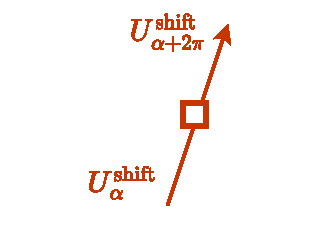
\includegraphics{figures/shift_2pi_isom.pdf}
\end{center}
\end{minipage}%
%
\begin{minipage}{0.50\linewidth}
\begin{center}
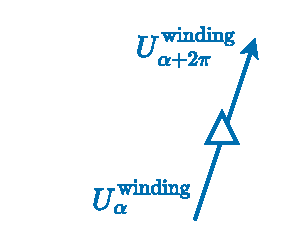
\includegraphics{figures/winding_2pi_isom.pdf}
\end{center}
\end{minipage}%

\caption{\label{fig-line-isom}Line-isomorphism operators.}

\end{figure}%

Likewise, the line isomorphism operator for the winding symmetry
operator is \[
 \exp\left(\imunit \alpha \int^{\triangle} \frac{d\phi}{2\pi} + \imunit\phi(\triangle)  + \imunit (\alpha+2\pi)  \int_{\triangle} \frac{d\phi}{2\pi}  \right).
\]

We let the composition of the two lines be denoted by
\(U_{\alpha,\beta} = U^\text{shift}_\alpha U^\text{winding}_\beta\).
With it, we can define ``naive'' junction where two line operators
\(U_{\alpha_1,\beta_1}\) and \(U_{\alpha_2,\beta_2}\) fusing into
\(U_{\alpha_1+\alpha_2,\beta_1+\beta_2}\). However, the fused operator
in general has parameters in the fundamental domain other than those of
the fused ones. Therefore, we normalize the junction by using the
\(\square\) and \(\triangle\) isomorphisms so that the output is
\(U_{\langle \alpha_1+\alpha_2\rangle, \langle \beta_1+\beta_2\rangle}\),
where \(\langle \alpha \rangle = 2\pi\{\alpha/2\pi\}\); see
Figure~\ref{fig-junction-def}. The point is that this isomorphism
results in a phase when crossing an intersection of the lines.

\begin{figure}[t]

\begin{minipage}{0.35\linewidth}
\begin{center}
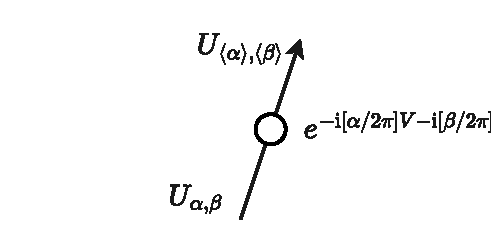
\includegraphics{figures/prod_isom.pdf}
\end{center}
\end{minipage}%
%
\begin{minipage}{0.05\linewidth}
~\end{minipage}%
%
\begin{minipage}{0.60\linewidth}
\begin{center}
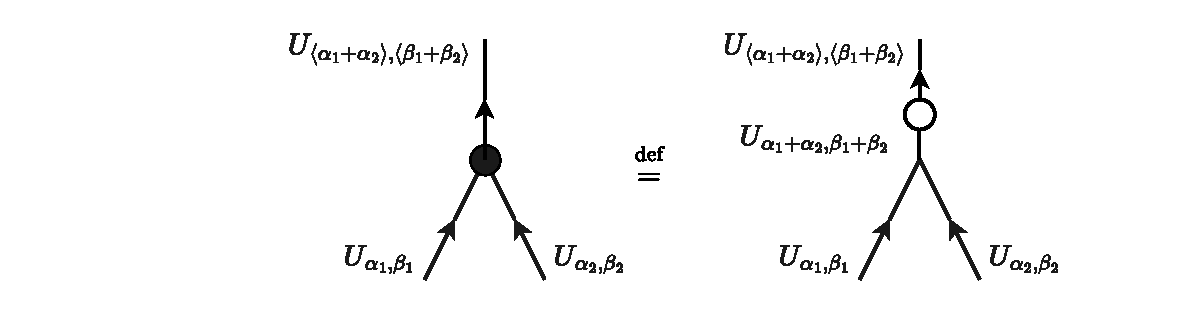
\includegraphics{figures/junction_def.pdf}
\end{center}
\end{minipage}%

\caption{\label{fig-junction-def}The definition of junction fusing two
\(U_{\alpha,\beta}\)'s into one.}

\end{figure}%

Now, we consider the two consecutive junctions, which fuses three lines
\(U_{\langle\alpha_i\rangle,\langle\beta_i\rangle}\) (\(i=1,2,3\)) into
\(U_{\langle\sum_i \alpha_i\rangle,\langle\sum_j \beta_j \rangle}\); see
Figure~\ref{fig-F-move}.

\begin{figure}[t]

\centering{

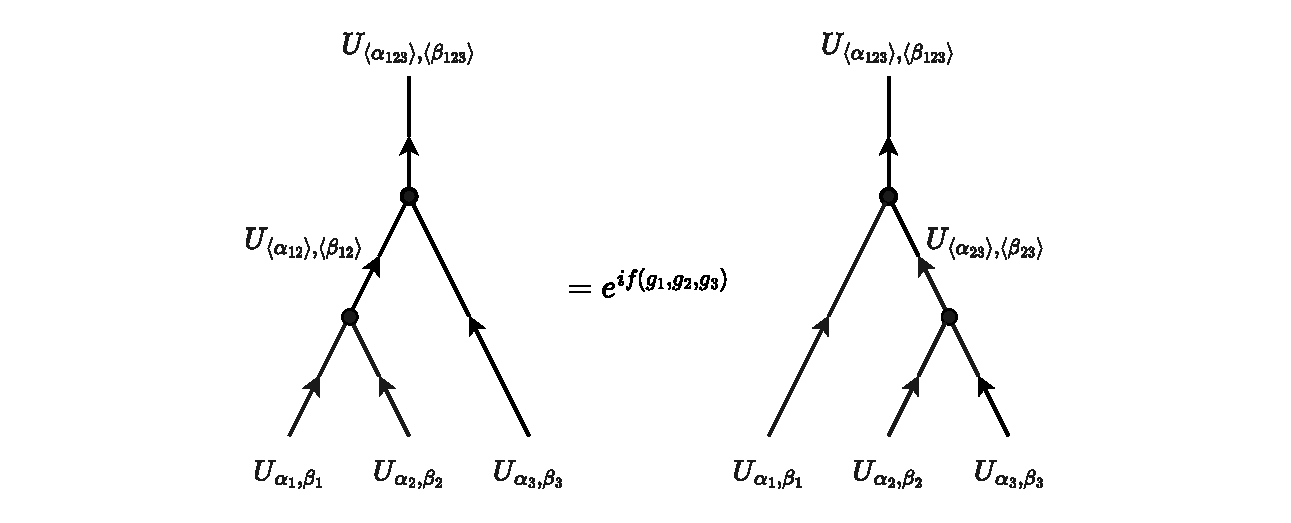
\includegraphics{figures/f_move.pdf}

}

\caption{\label{fig-F-move}The anomalous phase from the F-move. We let
\(\alpha_{12} = \alpha_1+\alpha_2\), etc.}

\end{figure}%

There are two ways of such fusion as depicted in the figure, and the two
are related by a nontrivial phase which is
\begin{equation}\phantomsection\label{eq-cocycle-boson}{
f(g_1,g_2,g_3) = \alpha_1\left[\frac{\langle\beta_2\rangle}{2\pi}+\frac{\langle\beta_3\rangle}{2\pi}\right]+\beta_3\left[\frac{\langle\alpha_1\rangle}{2\pi}+\frac{\langle\alpha_2\rangle}{2\pi}\right],
}\end{equation} where \(g_i = (\alpha_i,\beta_i)\in U(1)^2\). The two
configurations are gauge-equivalent, yet there is a non-trivial phase
relating them. This is the \emph{anomalous phase} of this anomalous
\(U(1)^2\) symmetry of 1+1d compact boson.

\begin{tcolorbox}[enhanced jigsaw, opacitybacktitle=0.6, titlerule=0mm, left=2mm, rightrule=.15mm, colbacktitle=quarto-callout-note-color!10!white, coltitle=black, breakable, leftrule=.75mm, bottomtitle=1mm, colback=white, colframe=quarto-callout-note-color-frame, toptitle=1mm, bottomrule=.15mm, opacityback=0, arc=.35mm, title=\textcolor{quarto-callout-note-color}{\faInfo}\hspace{0.5em}{Group cohomology}, toprule=.15mm]

Mathematically speaking, the function
\(f : (U(1)^2)^3 \to \mathbb{R}/2\pi\mathbb{Z}\) is a 3-cocycle on the
group \(G=U(1)^2\); it satisfies the \emph{pentagon identity}, depicted
in \textbf{?@fig-pentagon}.

Futher, it is subject to an ambiguity; we can modify the junction by a
phase \(h(g_1,g_2)\). This modifies the anomalous phase \(f\) as
\[ f(g_1,g_2,g_3) \mapsto f(g_1,g_2,g_3) + (\delta h)(g_1,g_2,g_3)
\] where \(\delta h : (U(1))^3\to \mathbb{R}/2\pi\mathbb{Z}\) is the
following function called a \emph{coboundary} (FIXME:sign?): \[
(\delta h)(g_1,g_2,g_3) = h(g_1,g_2) + h(g_1g_2,g_3) - h(g_1,g_2g_3) - h(g_2,g_3).
\] The third \textbf{group cohomology} is an element of the quatient
group \[
H^3 = \{f\in\Map(G^3,\mathbb{R}/2\pi\mathbb{Z})\mid\text{pentagon eq.}\} / \delta(\Map(G^3,\mathbb{R}/2\pi\mathbb{Z})),
\] where \(\Map(X,Y)\) is the abelian group of \(Y\) valued functions on
\(X\) \footnotemark{}. This group cohomology classifies the anomalous
phases of 1+1-dimensional bosonic theories with \(G\)-symmetry.

\end{tcolorbox}

\footnotetext{When \(G\) is continuous, the definition of
\(\Map(G^n,\mathbb{R}/2\pi\mathbb{Z})\) is subtle. The particular
cocycle \(f\) in Equation~\ref{eq-cocycle-boson} is not continuous, so
we do not want \(\Map(X,Y)\) to mean continuous maps. On the other hand
arbitrary discontinuous maps would contain too wild cocycles to be
realized in a QFT. In this particular case it seems considering
\emph{piecewise continuous} functions is necessary and sufficient. For
general cases in general dimensions KO is not sure.}

\begin{tcolorbox}[enhanced jigsaw, opacitybacktitle=0.6, titlerule=0mm, left=2mm, rightrule=.15mm, colbacktitle=quarto-callout-tip-color!10!white, coltitle=black, breakable, leftrule=.75mm, bottomtitle=1mm, colback=white, colframe=quarto-callout-tip-color-frame, toptitle=1mm, bottomrule=.15mm, opacityback=0, arc=.35mm, title=\textcolor{quarto-callout-tip-color}{\faLightbulb}\hspace{0.5em}{Exercise: \(\mathbb{Z}_2\) anomaly}, toprule=.15mm]

The diagonal \(\mathbb{Z}_3\) subgroup of \(U(1)^2\) generate by
\(U_{2\pi/3,2\pi/3}\) is anomalous. Confirm this fact by calculating
\(f(g_1,g_2,g_3)\) for \(g_i\)'s in this subgroup, and also proving that
no \(h\) can satisfy \(f = -\delta(h)\). Optionally one might consider
some other finite subgroups of \(U(1)^2\).

\end{tcolorbox}

\begin{tcolorbox}[enhanced jigsaw, opacitybacktitle=0.6, titlerule=0mm, left=2mm, rightrule=.15mm, colbacktitle=quarto-callout-note-color!10!white, coltitle=black, breakable, leftrule=.75mm, bottomtitle=1mm, colback=white, colframe=quarto-callout-note-color-frame, toptitle=1mm, bottomrule=.15mm, opacityback=0, arc=.35mm, title=\textcolor{quarto-callout-note-color}{\faInfo}\hspace{0.5em}{Comparison to more conventional calculation.}, toprule=.15mm]

The mixed anomaly between the shift and winding symmetry in 1+1d compact
boson is usually computed from the two-point function of the
corresponding current operators. Such computation corresopnds to
\emph{non-flat} and infinitesimal background for the symmetries. On the
other hand, inserting topological operator corresponds to \emph{flat}
and finite background. The two computations results in the same result
is quite non-trivial, and is explained by the Chern-Weil theory.

While the computation based on non-flat background is easier, it is only
for continuous symmetries and not obvious how it restricts to a finite
subgroup, for example.

\end{tcolorbox}

\section{T-duality}\label{sec-Tdual}

The compact boson in \(\stdim=2\)-dimensions famously has
\emph{T-duality}.

The T-duality is equivalence between the compact boson with radius \(R\)
and radius \(\frac{1}{R}\), and maps the shift (or momentum) symmetry of
one side to the winding symmetry of the other side, and vise versa. Note
that this makes sense because in \(\stdim=2\) the winding symmetry is a
0-form symmetry.

When the radius is the self-dual radius \(R=1\), the duality becomes a
(conventional) \(\mathbb{Z}_2\) symmetry, which is a part of the larger
emergent \(\SU(2)\) symmetry.

In this section we study

\begin{enumerate}
\def\labelenumi{\arabic{enumi}.}
\tightlist
\item
  the explicit construction of the T-duality topological interface
  connecting radius \(R\) and \(1/R\) theories
  \autocite{Kapustin:2009av}, and
\item
  its generalization giving \textbf{non-invertible} symmetry
  (i.e.~self-dual topological interface) at \(R=\sqrt{N}\) for an
  integer \(N\).
\end{enumerate}

The latter can further be generalized to the case of rational \(R^2\)
\autocite{Niro:2022ctq,Cordova:2023ent}.

\subsection{T-duality topological
interface}\label{t-duality-topological-interface}

Here we study the T-duality topological interface connecting two compact
boson theories in \(\stdim=2\)-dimensions; with radius \(R\) and radius
\(1/R\). \textbf{FIXME:figure!} When \(R=1\), the interface is a
topological operator within the same thoery, and thus defines a
symmetry. In this case it turns out a \(\mathbb{Z}_2\) symmetry, known
to be contained in the larger \(\SU(2)\) enhanced symmetry.

According to \autocite{Kapustin:2009av}, the partition functino
involving the interface is
\begin{equation}\phantomsection\label{eq-T-interface}{
\begin{multlined}
\langle \mathcal{O}_L \mathcal{I}^\text{T}_1[W] \mathcal{O}_R  \rangle= 
\int \mathop{\mathcal{D}^{M_L}\phi_L}\mathop{\mathcal{D}^{M_R}\phi_R}
\mathcal{O}_L[\phi_L]\mathcal{O}_R[\phi_R]\\
\exp\left(-\frac{R^2}{4\pi}\int_{M_L}\mathop{d\phi_L}*\mathop{d\phi_L}
-\frac{\imunit}{2\pi}\int_W \phi_L\mathop{d\phi_R}
-\frac{1}{4\pi R^2}\int_{M_R}\mathop{d\phi_R}*\mathop{d\phi_R}\right).
\end{multlined}
}\end{equation} For simplicity let us take \(\mathcal{O}_R =1\), and
\(M_R\) be a compact region in the spacetime. In this case, we expect
the supposed topological-ness implies \[
\langle \mathcal{O}_L \mathcal{I}_1^\text{T}[W]\rangle = \langle \mathcal{O}_L \rangle.
\] To show this, we replace the variable \(\phi_R\) with
\(F_R = d\phi_R\) by \[
\int \mathcal{D}\phi_R = \int \mathop{\mathcal{D}F_R} \mathop{\mathcal{D}\widetilde{\phi}_R}
\exp\left(\frac{\imunit}{2\pi} \int_{M_R}\widetilde{\phi}_R \mathop{dF_R}\right),
\] where the periodic scalar \(\widetilde{\phi}_R\) is the Lagrange
multiplier enforcing the closedness and the quantization of
\(F_R = d\phi_R\). Substituting this into Equation~\ref{eq-T-interface},
the EOMs with respect to \(F_R\) are
\begin{equation}\phantomsection\label{eq-EOM-FR-boson}{
\begin{aligned}
    \frac{1}{R} *d\phi_R(x) &= \imunit d\widetilde\phi_R(x) \quad \mathop{\text{for}} x \in M_R \\
    \phi_L(x) &= \widetilde{\phi}_R(x) \quad \mathop{\text{for}} x \in W.
\end{aligned}
}\end{equation} Substituting the former equation to the Lagrangea of
\(\phi_R\), we get \[
    \frac{R^2}{4\pi} \int_{M_R}\mathop{d\widetilde{\phi}_R}*\mathop{d\widetilde{\phi}_R}
\] with is the same as for \(\phi_L\), while the latter of
Equation~\ref{eq-EOM-FR-boson} connects \(\phi_L\) and
\(\widetilde{\phi}_R\) along \(W\). As a whole, we recover the
path-integral over \(M\) resulting in \(\langle \mathcal{O}_L \rangle\).
For a more general topological-ness about local deformation of \(W\) can
be derived in the same way but with more letters.

Now, let us set \(\mathcal{O}_R = \mathcal{O}^\text{winding}_n(x)\) and
see how the topological interface acts on the operator. As the operator
\(\mathcal{O}^\text{winding}_n\) in Equation~\ref{eq-dual-op} is defined
on the trivial surface operator, we have to divide the manifold into
three parts: \(M_L,M_M,m_R\), separated by \(W_1\) and \(W_2\). As the
\(M_L\) and field on it is not going to be relevant, we suppress them in
the following equations. The calculation goes as:

\[
\begin{aligned}
\mathcal{I}_1^\text{T} \mathcal{O}^\text{winding}_n(x)
&= \int \mathop{\mathcal{D}\phi_M}\mathop{\mathcal{D}\phi_R}\mathop{\mathcal{D}^{W_2}V}
\exp\left(-S_M^{1/R}-S_R^{1/R}-\frac{\imunit}{2\pi}\int_{W_1}\phi_L \mathop{d\phi_M}\right)\\
 &\times\exp\left(\frac{\imunit}{2\pi}\int_{W_2}\mathop{dV}(\phi_M-\phi_R) + \imunit n V(x) \right)\\
&= \int \mathop{\mathcal{D}F_M}\mathop{\mathcal{D}F_R}\mathop{\mathcal{D}^{W_2}V}\mathop{\mathcal{D}\widetilde\phi_M}\mathop{\mathcal{D}\widetilde\phi_R}\\
&\times\exp\left(-S_M^{1/R}-S_R^{1/R}-\frac{\imunit}{2\pi}(\int_{W_1}\phi_L \mathop{d\phi_M}-\int_{M_M}\tilde{\phi}_M\mathop{dF_M} - \int_{M_R}\tilde{\phi}_R\mathop{dF_R})\right)\\
 &\times\exp\left(+\frac{\imunit}{2\pi}\int_{W_2}\mathop{V}(F_M-F_R) + \imunit n V(x) \right)
\end{aligned}
\] Now, the EOMs in terms of \(F_M\) and \(F_R\) state \[
\begin{aligned}
    \frac{1}{R} *d\phi_{M,R} &= \imunit d\widetilde\phi_{M,R}(x) \quad \text{on} \;\; M_{M,R}, \\
    \phi_L &= \widetilde{\phi}_M \quad \text{on} \;\; W_1,\\
\tilde{\phi}_M &= V = \tilde{\phi}_R \quad \text{on} \;\; W_2.
\end{aligned}
\] Thus by substituting back we get \textbf{FIXME:check the sign!} \[
\mathcal{I}_1^\text{T}\cdots\mathcal{O}_n^\text{winding} = \mathcal{O}_{\pm? n}^\text{shift}.
\]

In addition, let us calculate \((\mathcal{I}_1[W]^\text{T})^2\). For
this, we insert the defects along parallel submanifolds \(W_1\) and
\(W_2\) and take the limit where the separation of the two shrinks.
\textbf{FIXME:figure} This can be calculated as \[
\begin{aligned}
\mathcal{I}_1^\text{T}[W_1]\mathcal{I}_1^\text{T}[W_2]
&= \int \mathcal{D}^{M_M}\phi_M \exp(-\imunit \int_{W_1} \phi_L d\phi_M - \imunit\int_{W_2} \phi_M d\phi_R)\\
&= \int \mathcal{D}^{W}\phi_M \exp(-\imunit \int_{W} (\phi_L - \phi_R) d\phi_M)\\
&= \id[W],
\end{aligned}
\] where in the second line we collide \(W_1\) and \(W_2\), and noted
that only the mode of \(\phi_M\) constant along the direction
perpendicular to \(W_1\) and \(W_2\) contributes. Therefore, the
T-duality interface squares to the identity. In particular, at \(R=1\),
the self-interface defines an invertible \(\mathbb{Z}_2\) symmetry.

\subsection{Non-invertible symmetry from
T-duality}\label{non-invertible-symmetry-from-t-duality}

\textcite{Choi:2021kmx} generalized the Kapustin-Tikhonov T-duality
interface by \textcite{Kapustin:2009av} as
\begin{equation}\phantomsection\label{eq-TN-interface}{
\begin{multlined}
\langle \mathcal{O}_L \mathcal{I}^\text{T}_N[W] \mathcal{O}_R  \rangle= 
\int \mathop{\mathcal{D}^{M_L}\phi_L}\mathop{\mathcal{D}^{M_R}\phi_R}
\mathcal{O}_L[\phi_L]\mathcal{O}_R[\phi_R]\\
\exp\left(-\frac{R^2}{4\pi}\int_{M_L}\mathop{d\phi_L}*\mathop{d\phi_L}
-\frac{\imunit N}{2\pi}\int_W \phi_L\mathop{d\phi_R}
-\frac{N^2}{4\pi R^2}\int_{M_R}\mathop{d\phi_R}*\mathop{d\phi_R}\right).
\end{multlined}
}\end{equation} This interface is a \emph{self-interface} at
\(R=\sqrt{N}\). The same procedure as we did for \(\mathcal{I}_1\) leads
to \begin{equation}\phantomsection\label{eq-TN-interface2}{
\begin{multlined}
\langle\mathcal{O}_L \mathcal{I}^\text{T}_N[W] \rangle= 
\int \mathop{\mathcal{D}^{M_L}\phi_L}\mathop{\mathcal{D}^{M_R}\phi_R}\mathop{\mathcal{D}^{W}V'}
\mathcal{O}_L[\phi_L]\\
\exp\left(-\frac{R^2}{4\pi}\int_{M_L}\mathop{d\phi_L}*\mathop{d\phi_L}
-\frac{\imunit }{2\pi}\int_W (N \phi_L - \widetilde{\phi}_R)\mathop{dV}
-\frac{R^2}{4\pi N^2}\int_{M_R}\mathop{d\widetilde\phi_R}*\mathop{d\widetilde\phi_R}\right).
\end{multlined}
}\end{equation} We further rescale the fields as

\[
\begin{aligned}
V' &= NV \\
N \widetilde\phi_R' &= \widetilde\phi_R \mod 2\pi
\end{aligned}
\] so that we have
\begin{equation}\phantomsection\label{eq-TN-interface3}{
\begin{multlined}
\langle\mathcal{O}_L \mathcal{I}^\text{T}_N[W] \rangle = \mathcal{N} 
\int \mathop{\mathcal{D}^{M_L}\phi_L}\mathop{\mathcal{D}^{M_R}\phi_R}\mathop{\mathcal{D}^{W}V'}
\mathcal{O}_L[\phi_L]\\
\exp\left(-\frac{R^2}{4\pi}\int_{M_L}\mathop{d\phi_L}*\mathop{d\phi_L}
-\frac{\imunit }{2\pi}\int_W ( \phi_L - \widetilde{\phi}_R')\mathop{dV'}
-\frac{R^2}{4\pi}\int_{M_R}\mathop{d\widetilde\phi_R'}*\mathop{d\widetilde\phi_R'}\right).
\end{multlined}
}\end{equation} To go from Equation~\ref{eq-TN-interface3} to
Equation~\ref{eq-TN-interface2}, we define a \(\mathbb{Z}_N\) valued
variable
\(n_{\widetilde{\phi'}_R} = [N\widetilde{\phi'}_R/2\pi] \mod N\) so that
\(\widetilde{\phi'} = \frac{2\pi}{N}(\{\widetilde{\phi}/2\pi\} + 2\pi n_{\widetilde{\phi'}_R})\).
Then, after substituting it, the sum over \(n_{\widetilde{\phi'}}\)
enforces \(V'\) be divisible by \(N\) (that is, the winding of \(V\)
along \(W\) is constrained to be a multiple of \(N\)). Thus, we have
\[\langle\mathcal{O}_L \mathcal{I}_N^\text{T}[W]\rangle = \mathcal{N} \langle \mathcal{O}_L \rangle.
\] We are not caring enough about the absolute size of path-integral
measure to determine the normalization constant \(\mathcal{N}\), but
will determined in by another mean later.

\subsubsection{Fusion rule}\label{fusion-rule}

The product, or \emph{fusion} of the generalized operator is
\begin{equation}\phantomsection\label{eq-fusion-I}{
\begin{aligned}
(\mathcal{I}_N^\text{T})^2 &= \int \mathcal{D}^W V \exp(\frac{\imunit}{2\pi} N \int_W \mathop{dV}(\phi_L-\phi_R))\\
&= \sum_{n=0}^{N-1} \int \mathcal{D}^W V' \exp(\frac{\imunit}{2\pi}  \int_W \mathop{dV}(\phi_L-\phi_R+ 2\pi n/N))\\
&= \sum_{n=0}^{N-1} U_{2\pi n/N}^{\text{shift}},
\end{aligned}
}\end{equation} where in the second line we did the chage of variable
\(NV = V'\), and enforced the divisibility of \(V'\) by \(N\) by the sum
over \(n\). One can also see
\(\mathcal{I}_N^\text{T}[-W] = \mathcal{I}_N^\text{T}[W]\) (note that
when we consider an operator on \(W\) the notion of ``left'' and
``right'' also flips), so \[
\mathcal{I}_N^\text{T}[W]\mathcal{I}_N^\text{T}[-W] = \sum_{n=0}^{N-1} U_{2\pi n/N}^{\text{shift}}.
\] This contrasts to the case of conventional symmetry operator, where
\(U_g[W] = U_{g^{-1}}[W]\) and thus \[
U_g [W] U_g[-W] = \id[W].
\] In the case of \(\mathcal{I}_N^\text{T}\), \(N\ge 2\), the fusion
with its orientation reversal is not the trivial operator, but a sum.
This is a one of hallmarks of \textbf{non-invertible} symmetry.
\(\mathcal{I}_N^\text{T}[-W]\), called the \textbf{dual} of the original
operator, is the closest possible thing to be the ``inverse'', but it
fails to be so. Therefore, the compact boson theory in 1+1d at
\(R=\sqrt{N}\) has the non-invertible T-duality symmetry.

Here, we can determine that the coefficient in the above equations are
correct. This is because that we can insert the one-dimensional operator
\((\mathcal{I}_N^\text{T})^2\) along the time direction, which should
determine the \emph{defect Hilbert} space. On the right hand side, we
should have a direct sum of defect Hilbert spaces for the involved
invertible symmetry operators. There is no way to take ``average'' over
Hilbert spaces, or divide it by a number, so we can assume the minimal
possible coefficient is realized, which is the one in
Equation~\ref{eq-fusion-I}.

Given Equation~\ref{eq-fusion-I}, the coefficient \(\mathcal{N}\) in
Equation~\ref{eq-TN-interface3} is determined by \[
\langle (\mathcal{I}_N^\text{T})^2[W] \rangle = \sum_{n=0}^{N-1}\langle U_{2\pi n/N}^\text{shift}[W] \rangle = \mathcal{N}^2,
\] thus \(\mathcal{N} = \sqrt{N}\). This quantity is called the
\textbf{quantum dimension} of \(\mathcal{I}_N^\text{T}\).

\subsubsection{Action on the local
operators}\label{action-on-the-local-operators}

What is the action of \(\mathcal{I}_N^\text{T}\) on the local operator
\(\mathcal{O}^\text{winding}_n\)? Naively repeating the procedure in the
previous section, one might think \[
\mathcal{I}_N^\text{T} \cdot \mathcal{O}^\text{winding}_n(x) \stackrel{?}{=} \mathcal{O}^\text{shift}_{n/N}(x)
\] however the left hand side, \(e^{\imunit n/N \phi}\), does not make
sense when \(N\) does not divide \(n\) as it is incompatible with the
periodicity of \(\phi\). Thus the right hand side vanishes unless
\(N | n\), and we have \[
\mathcal{I}_N^\text{T} \cdot \mathcal{O}^\text{winding}_n(x) = 
\begin{cases}
e^{\imunit \frac{n}{N}\phi} & N|n \\
0 & \text{otherwise}.
\end{cases}
\] Note that here we considered the \emph{encircling} action
(FIXME:Figure!!). We can instead consider the \emph{passing} action, in
which case we have \[
\mathcal{I}_N^\text{T}[W_L]  \mathcal{O}^\text{winding}_n(x) = 
e^{\imunit \frac{n}{N}\int_{\gamma^x} \mathop{d\phi}} \mathcal{I}_N^\text{T}[W_R],
\] \(W_{L,R}\) goes through the left/right side of the point \(x\), and
the path \(\gamma^x\) starts from a point on \(W_R\) and ends at \(x\).

\subsection{\texorpdfstring{Non-invertible T-duality for a rational
\(R\)}{Non-invertible T-duality for a rational R}}\label{non-invertible-t-duality-for-a-rational-r}

We can further generalize Equation~\ref{eq-TN-interface} so that it is a
self duality at \(R^2 = p/q\) (\(p\) and \(q\) are taken to be coprime)
\autocite{Niro:2022ctq,Cordova:2023ent}. The construction is \[
\mathcal{I}_{p,q}^\text{T}[W]=\int \mathop{\mathcal{D}^W a} \mathop{\mathcal{D}^W b} \exp\left(-\frac{\imunit}{2\pi}  \int_W (q \mathop{a} \mathop{db} +p \mathop{a} \mathop{d\phi_L} - b \mathop{d\phi_R} )\right),
\] where \(a\) and \(b\) are periodic scalar fields on \(W\). The fusion
is \[
(\mathcal{I}_{p,q}^\text{T}[W])^2 = \sum_{n_1=0}^{p-1}\sum_{n_2=0}^{q-1}U^\text{shift}_{2\pi n_1/N}U^\text{winding}_{2\pi n_2/N},
\] and the quantum dimension is \[
\langle \mathcal{I}_{p,q}^\text{T}[W]\rangle = \sqrt{pq}.
\]

\bookmarksetup{startatroot}

\chapter{Vector}\label{sec-vector}

\bookmarksetup{startatroot}

\chapter*{References}\label{references}
\addcontentsline{toc}{chapter}{References}

\markboth{References}{References}

\printbibliography[heading=none]

\cleardoublepage
\phantomsection
\addcontentsline{toc}{part}{Appendices}
\appendix

\chapter{Classical Symmetry in Sigma Model and equivariant
cohomology}\label{sec-equivariant}

In Chapter~\ref{sec-scalar} we saw that the symmetry transformation by
\(g \in G\) of the Lagrangian (density) can acompany a surface turm
\(ds(\phi,g)\) with some \((D-1)\)-form \(s(\phi,g)\). Further, the
assosiativity of the transformations imply that we have
Equation~\ref{eq-surface-term-assosiative} (repeating here)
\begin{equation}\phantomsection\label{eq-surface-term-assosiative-app}{ 
s(\phi^{g_1},g_2) + s(\phi,g_1) = s(\phi,g_2g_1) + ds^{(1)}(\phi,g_1,g_2)
}\end{equation} with some \((D-2)\) forms \(s^{(1)}(\phi,g_1,g_2)\).

This structure continues when \(D\ge 2\). At the next level,

As the reader might have expected, the structure regarding \(s\) and
\(s^{(1)}\) continues: there are \((D-3)\)-forms
\(s^{(2)}(\phi,g_1,g_2,g_3)\) governing the ``\emph{higher
associativity}'' among \(s^{(1)}\), and so on, until
\(s^{(D-1)}(\phi,g_1,g_2,\cdots,g_{D})\) that are 0-forms. Although we
consider the free scalar fields these higher surface terms can be taken
to be zero and irrelevant, it might not be the case when we consider a
sigma model with target \(X\) with a non-trivial topology.

Let \(s^{(-1)}\) be the metric independent part of \(\mathcal{L}\), and
\(s^{(0)}=s\). The tuple \((s^{(-1)},s^{(0)},\cdots,s^{(D-1)})\)
defineds an degree-\(D\) \textbf{equivariant cohomology class}
\(\mathbf{s} \in H_G^D(X)\). In other words \(G\)-symmetric topologicall
terms in \(X\)-target sigma model is classified by the \(G\)-equivariant
cohomology, when \(G\) is a classical symmetry acting on \(X\). The
model\footnote{The word ``model'' in mathematics, in particular homotopy
  theory, is used to indecate a concrete construction of an abstract
  mathematical concept. This usage might go in the opposite direction to
  the physicists' one: an abstraction of the (quasi-)real world.} of the
equivariant cohomology realized by \((s^{(-1)},s^{(0)},\cdots)\) is
called simplicial de Rham cohomology, see e.g.~@. Note that this model
works for discrete groups, as opposed to the Weyl model based on Lie
derivatives that applies to continuous groups.




\end{document}
